\documentclass[../main.tex]{subfiles}

\begin{document}
\chapter{Liniowo przekształcony rozkład kosinusowy}
\label{Chapter:LTC}

Metody przedstawione w poprzednich rozdziałach nie znajdowały rozwiązania dokładnego, a jedynie jego dobre przybliżenie. Innym sposobem wyznaczenia rozwiązania przybliżonego jest przekształcenie obliczanej funkcji, w taki sposób, aby miała ona bardzo podobny kształt, a jednak posiadała właściwości umożliwiające obliczenie wartości funkcji w sposób analityczny.

Autorzy \cite{ltc_heitz} zaproponowali znalezienie przybliżenia wyrażenia całkowego na wielokącie sferycznym $P$, reprezentującym światło powierzchniowe, postaci przedstawionej w równaniu (\ref{eq:ltc_render_approx}).
\begin{equation}
L_o(\omega_o) = \int_{P} {
  L_i(\omega_i)
  f_r(\omega_i, \omega_o)
  \cos \theta_i
  \dd \omega_i
}
\approx
\int_{P} {
  L_i(\omega_i)
  D_A(\omega_i)
  \dd \omega_i
}
\label{eq:ltc_render_approx}
\end{equation}

Wielokąt sferyczny $P$ możemy interpretować jako zbiór wszystkich kierunków promieni przecinających powierzchnię światła, wychodzących z analizowanego punktu.

Funkcję aproksymującą $D_A(\omega)$ \footnote{Funkcja $D_A(\omega)$ nie jest związana z z funkcją rozkładu normalnych $D(m)$, podobne oznaczenie zostało zachowane dla kompatybilności z pracą \cite{ltc_heitz}.} chcielibyśmy dobrać tak, aby całe wyrażenie posiadało wzór jawny lub było możliwe do obliczenia w bardzo krótkim czasie.

Autorzy pracy \cite{ltc_heitz} postanowili najpierw uprościć problem jeszcze bardziej i znaleźć taki rozkład, który można całkować niezależnie w czasie rzeczywistym i pozwala modelować zjawiska istotne dla funkcji BRDF. Z definicji spełnienie pierwszego warunku wymaga by dla danego rozkładu $D_A(\omega)$ całka  (\ref{eq:LTCDInt}) była możliwa do obliczenia w sposób analityczny.
\begin{equation}
\int_P {
    D_A(\omega)
    \dd \omega
}
\label{eq:LTCDInt}
\end{equation}

Zakładając znajomość rozwiązania całki (\ref{eq:LTCDInt}), uproszczenie (\ref{eq:ltc_render_approx}) pozwala nam na proste rozwiązanie przypadku dla światła o jednorodnym kolorze. W takiej sytuacji, jeżeli promień wysłany w kierunku $\omega$ przecina światło powierzchniowe $P$, to $L(\omega)=L$. W przeciwnym przypadku zachodzi $L(\omega)=0$. Zatem równanie (\ref{eq:ltc_render_approx}) możemy przepisać jako (\ref{ltc_render_approx_uniform_color}).
\begin{equation}
L_o(\omega_o) =
\int_{P} {
    L_i(\omega_i)
    D_A(\omega_i)
    \dd \omega_i
} = \int_{P} {
    L *
    D_A(\omega_i)
    \dd \omega_i
} = L \int_{P} {
    D_A(\omega_i)
    \dd \omega_i
}
\label{ltc_render_approx_uniform_color}
\end{equation}

\section{Wybór rozkładu aproksymującego $D_A(\omega)$}

Rozpocznijmy od zdefiniowania warunków, które funkcja $D_A(\omega)$ musi spełniać, aby nadawała się do zastosowania jako element przybliżenia. W zaawansowanych modelach oświetlenia bazowanych na zjawiskach fizycznych występuje kilka ważnych efektów, które muszą zostać zachowane. Ze względu na różnorodność materiałów występujących w typowej scenie, metoda musi wspierać zmienną chropowatość powierzchni określoną przez parametr $\alpha$.

Pierwszym z istotnych efektów jest odpowiedź funkcji BRDF dla powierzchni obserwowanych pod odpowiednio dużym kątem, która zostaje rozciągnięta wzdłuż jednej z osi formując kształt eliptyczny (rys. \ref{fig:BRDFGrazingAnisotropy}).

\begin{figure}
    \centering
    
    \begin{subfigure}[t]{0.18\textwidth}
        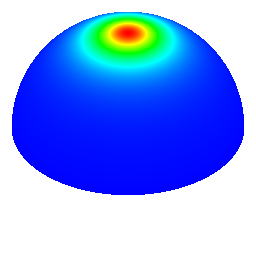
\includegraphics[width=\textwidth]{ltc/fit_r28_a0_brdf}
    \end{subfigure}
    \begin{subfigure}[t]{0.18\textwidth}
        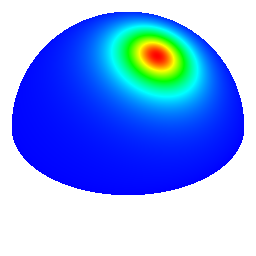
\includegraphics[width=\textwidth]{ltc/fit_r28_a16_brdf}
    \end{subfigure}
    \begin{subfigure}[t]{0.18\textwidth}
        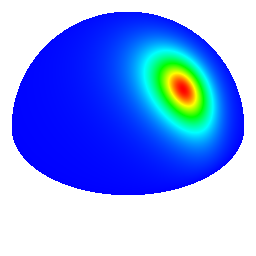
\includegraphics[width=\textwidth]{ltc/fit_r28_a32_brdf}
    \end{subfigure}
    \begin{subfigure}[t]{0.18\textwidth}
        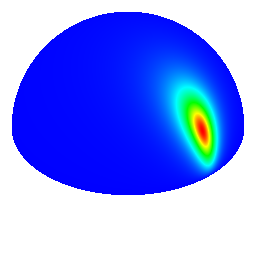
\includegraphics[width=\textwidth]{ltc/fit_r28_a48_brdf}
    \end{subfigure}
    \begin{subfigure}[t]{0.18\textwidth}
        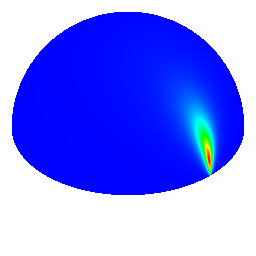
\includegraphics[width=\textwidth]{ltc/fit_r28_a60_brdf}
    \end{subfigure}
    
    \caption{Zjawisko rozciągnięcia odpowiedzi BRDF na jednej osi przy dużym kącie padania wiązki. Do wygnerowania podglądu wykorzystano model GGX. Opracowanie własne.}
    \label{fig:BRDFGrazingAnisotropy}
\end{figure}

Drugim efektem jest przesuwanie się maksimum rozproszenia bliżej normalnej, gdy przy dużym kącie obserwacji zwiększamy chropowatość materiału (rys. \ref{fig:BRDFOffSpecular}). Powyższe zjawisko jest znane jako maksimum poza kątem odbicia (ang. \textit{off-specular peak}).

\begin{figure}
    \centering
    
    \begin{subfigure}[t]{0.18\textwidth}
        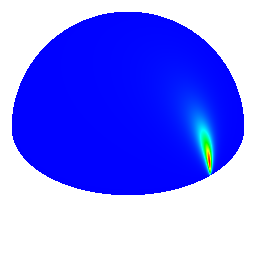
\includegraphics[width=\textwidth]{ltc/offspecular/fit_r25_a60_brdf}
    \end{subfigure}
    \begin{subfigure}[t]{0.18\textwidth}
        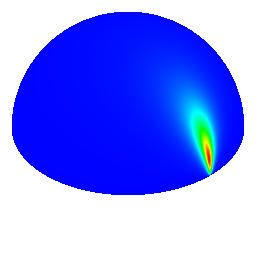
\includegraphics[width=\textwidth]{ltc/offspecular/fit_r30_a60_brdf}
    \end{subfigure}
    \begin{subfigure}[t]{0.18\textwidth}
        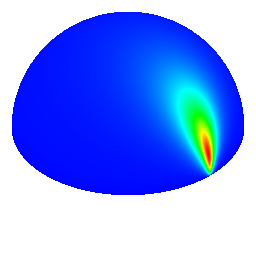
\includegraphics[width=\textwidth]{ltc/offspecular/fit_r35_a60_brdf}
    \end{subfigure}
    \begin{subfigure}[t]{0.18\textwidth}
        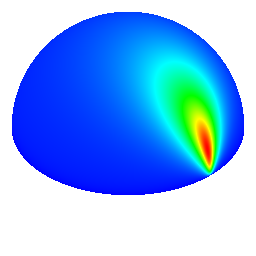
\includegraphics[width=\textwidth]{ltc/offspecular/fit_r40_a60_brdf}
    \end{subfigure}
    \begin{subfigure}[t]{0.18\textwidth}
        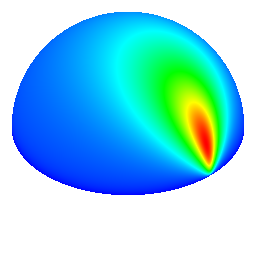
\includegraphics[width=\textwidth]{ltc/offspecular/fit_r45_a60_brdf}
    \end{subfigure}
    
    \caption{Zjawisko przesuwania się maksimum w kierunku normalnej. Do wygnerowania podglądu wykorzystano model GGX. Opracowanie własne.}
    \label{fig:BRDFOffSpecular}
\end{figure}

%\begin{figure}
%    \centering
%    
%    \begin{subfigure}[t]{0.3\textwidth}
%        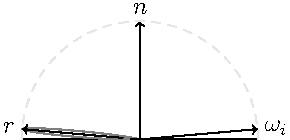
\includegraphics[width=\textwidth]{ltc/offspecular_0}
%        \caption{\ang{5} nachylenia, $\alpha = 0.2^2$}
%    \end{subfigure}
%    \begin{subfigure}[t]{0.3\textwidth}
%        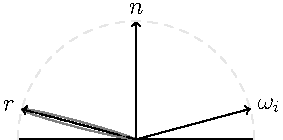
\includegraphics[width=\textwidth]{ltc/offspecular_1}
%        \caption{\ang{15} nachylenia, $\alpha = 0.2^2$}
%    \end{subfigure}
%    \begin{subfigure}[t]{0.3\textwidth}
%        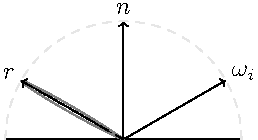
\includegraphics[width=\textwidth]{ltc/offspecular_2}
%        \caption{\ang{30} nachylenia, $\alpha = 0.2^2$}
%    \end{subfigure}
%
%    \begin{subfigure}[t]{0.3\textwidth}
%        \centering
%        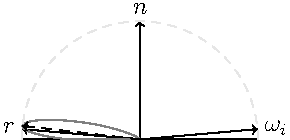
\includegraphics[width=\textwidth]{ltc/offspecular_3}
%        \caption{\ang{5} nachylenia, $\alpha = 0.4^2$}
%    \end{subfigure}
%    \begin{subfigure}[t]{0.3\textwidth}
%        \centering
%        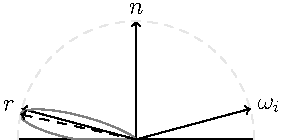
\includegraphics[width=\textwidth]{ltc/offspecular_4}
%        \caption{\ang{15} nachylenia, $\alpha = 0.4^2$}
%    \end{subfigure}
%    \begin{subfigure}[t]{0.3\textwidth}
%        \centering
%        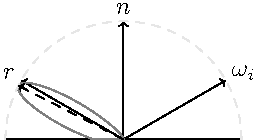
\includegraphics[width=\textwidth]{ltc/offspecular_5}
%        \caption{\ang{30} nachylenia, $\alpha = 0.4^2$}
%    \end{subfigure}
%
%    \begin{subfigure}[t]{0.3\textwidth}
%        \centering
%        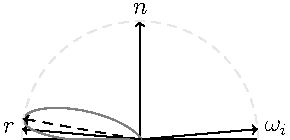
\includegraphics[width=\textwidth]{ltc/offspecular_6}
%        \caption{\ang{5} nachylenia, $\alpha = 0.6^2$}
%    \end{subfigure}
%    \begin{subfigure}[t]{0.3\textwidth}
%        \centering
%        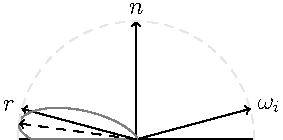
\includegraphics[width=\textwidth]{ltc/offspecular_7}
%        \caption{\ang{15} nachylenia, $\alpha = 0.6^2$}
%    \end{subfigure}
%    \begin{subfigure}[t]{0.3\textwidth}
%        \centering
%        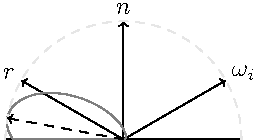
\includegraphics[width=\textwidth]{ltc/offspecular_8}
%        \caption{\ang{30} nachylenia, $\alpha = 0.6^2$}
%    \end{subfigure}
%
%    \begin{subfigure}[t]{0.3\textwidth}
%        \centering
%        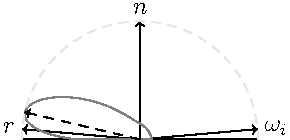
\includegraphics[width=\textwidth]{ltc/offspecular_9}
%        \caption{\ang{5} nachylenia, $\alpha = 0.8^2$}
%    \end{subfigure}
%    \begin{subfigure}[t]{0.3\textwidth}
%        \centering
%        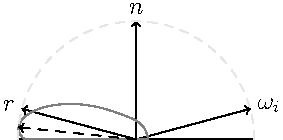
\includegraphics[width=\textwidth]{ltc/offspecular_10}
%        \caption{\ang{15} nachylenia, $\alpha = 0.8^2$}
%    \end{subfigure}
%    \begin{subfigure}[t]{0.3\textwidth}
%        \centering
%        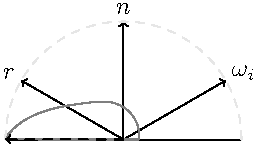
\includegraphics[width=\textwidth]{ltc/offspecular_11}
%        \caption{\ang{30} nachylenia, $\alpha = 0.8^2$}
%    \end{subfigure}
%    
%    \caption{Różnice między najsilniejszym kierunkiem odbicia od powierzchni o chropowatości $\sqrt{\alpha}$, a kierunkiem odbicia idealnego $r$. Do wygenerowania wykorzystano model GGX. Opracowanie własne.}
%    \label{fig:BRDFOffSpecular}
%\end{figure}

Warto zauważyć, że gdy $D_A(\omega)$ jest rozkładem gęstości prawdopodobieństwa to całka (\ref{eq:LTCDInt}) definiuje całkowite prawdopodobieństwo, że próbka wygenerowana z rozkładu $D_A$ przetnie wielokąt $P$. W takim przypadku, gdy korzystając z metody Monte-Carlo wielokrotnie wybierzemy losowy wektor z rozkładu $D_A(\omega)$ i sprawdzimy istnienie punktu przecięcia tego promienia z wielokątem $P$ to dla odpowiednio dużej liczby próbek stosunek trafień do ilości przetestowanych promieni będzie przybliżał naszą szukaną całkę.

Kluczową obserwacją jest to, że rozkład jest równoważny nieskończonej ilości próbek tego rozkładu. Każdą z tych form da się przekształcić na drugą w sposób bezpośredni i bezstratny. Zatem rozkład na sferze jest obiektem dualnym do nieskończonego zbioru ilości próbek tego samego rozkładu. Wynika z tego to, że po zmodyfikowaniu jednego otrzymamy nowy obiekt matematyczny, który potem będziemy mogli przekształcić w drugi.

Przykładem takiej operacji może być przekształcenie liniowe modyfikujące kierunek próbki. Będziemy zakładać, że próbka po przekształceniu liniowym w dalszym ciągu jest jednostkowej długości tzn. zawsze zostaje z powrotem znormalizowana. Takie przekształcenie ma kilka bardzo ważnych właściwości, które będziemy wykorzystywać. Warto zauważyć, że jeżeli przekształcimy rozkład prawdopodobieństwa przekształceniem $M$, to gdy zrobimy to samo z wielokątem $P$, otrzymując wielokąt $P^\prime$, prawdopodobieństwo, że nowa próbka przetnie nowy wielokąt nie zmieni się. Widać to wyraźnie z faktu, że przekształcone próbki podążają za przekształcanym wielokątem. Zachodzi więc równość (\ref{fig:LTCTransformEquality}).
\begin{equation}
\int_P {
  D_A(\omega)
  \dd \omega
} = \int_{P^\prime} {
  D^\prime_A(\omega)
  \dd \omega
}
\label{fig:LTCTransformEquality}
\end{equation}

\begin{figure}
    \centering
    \begin{subfigure}[t]{0.45\textwidth}
        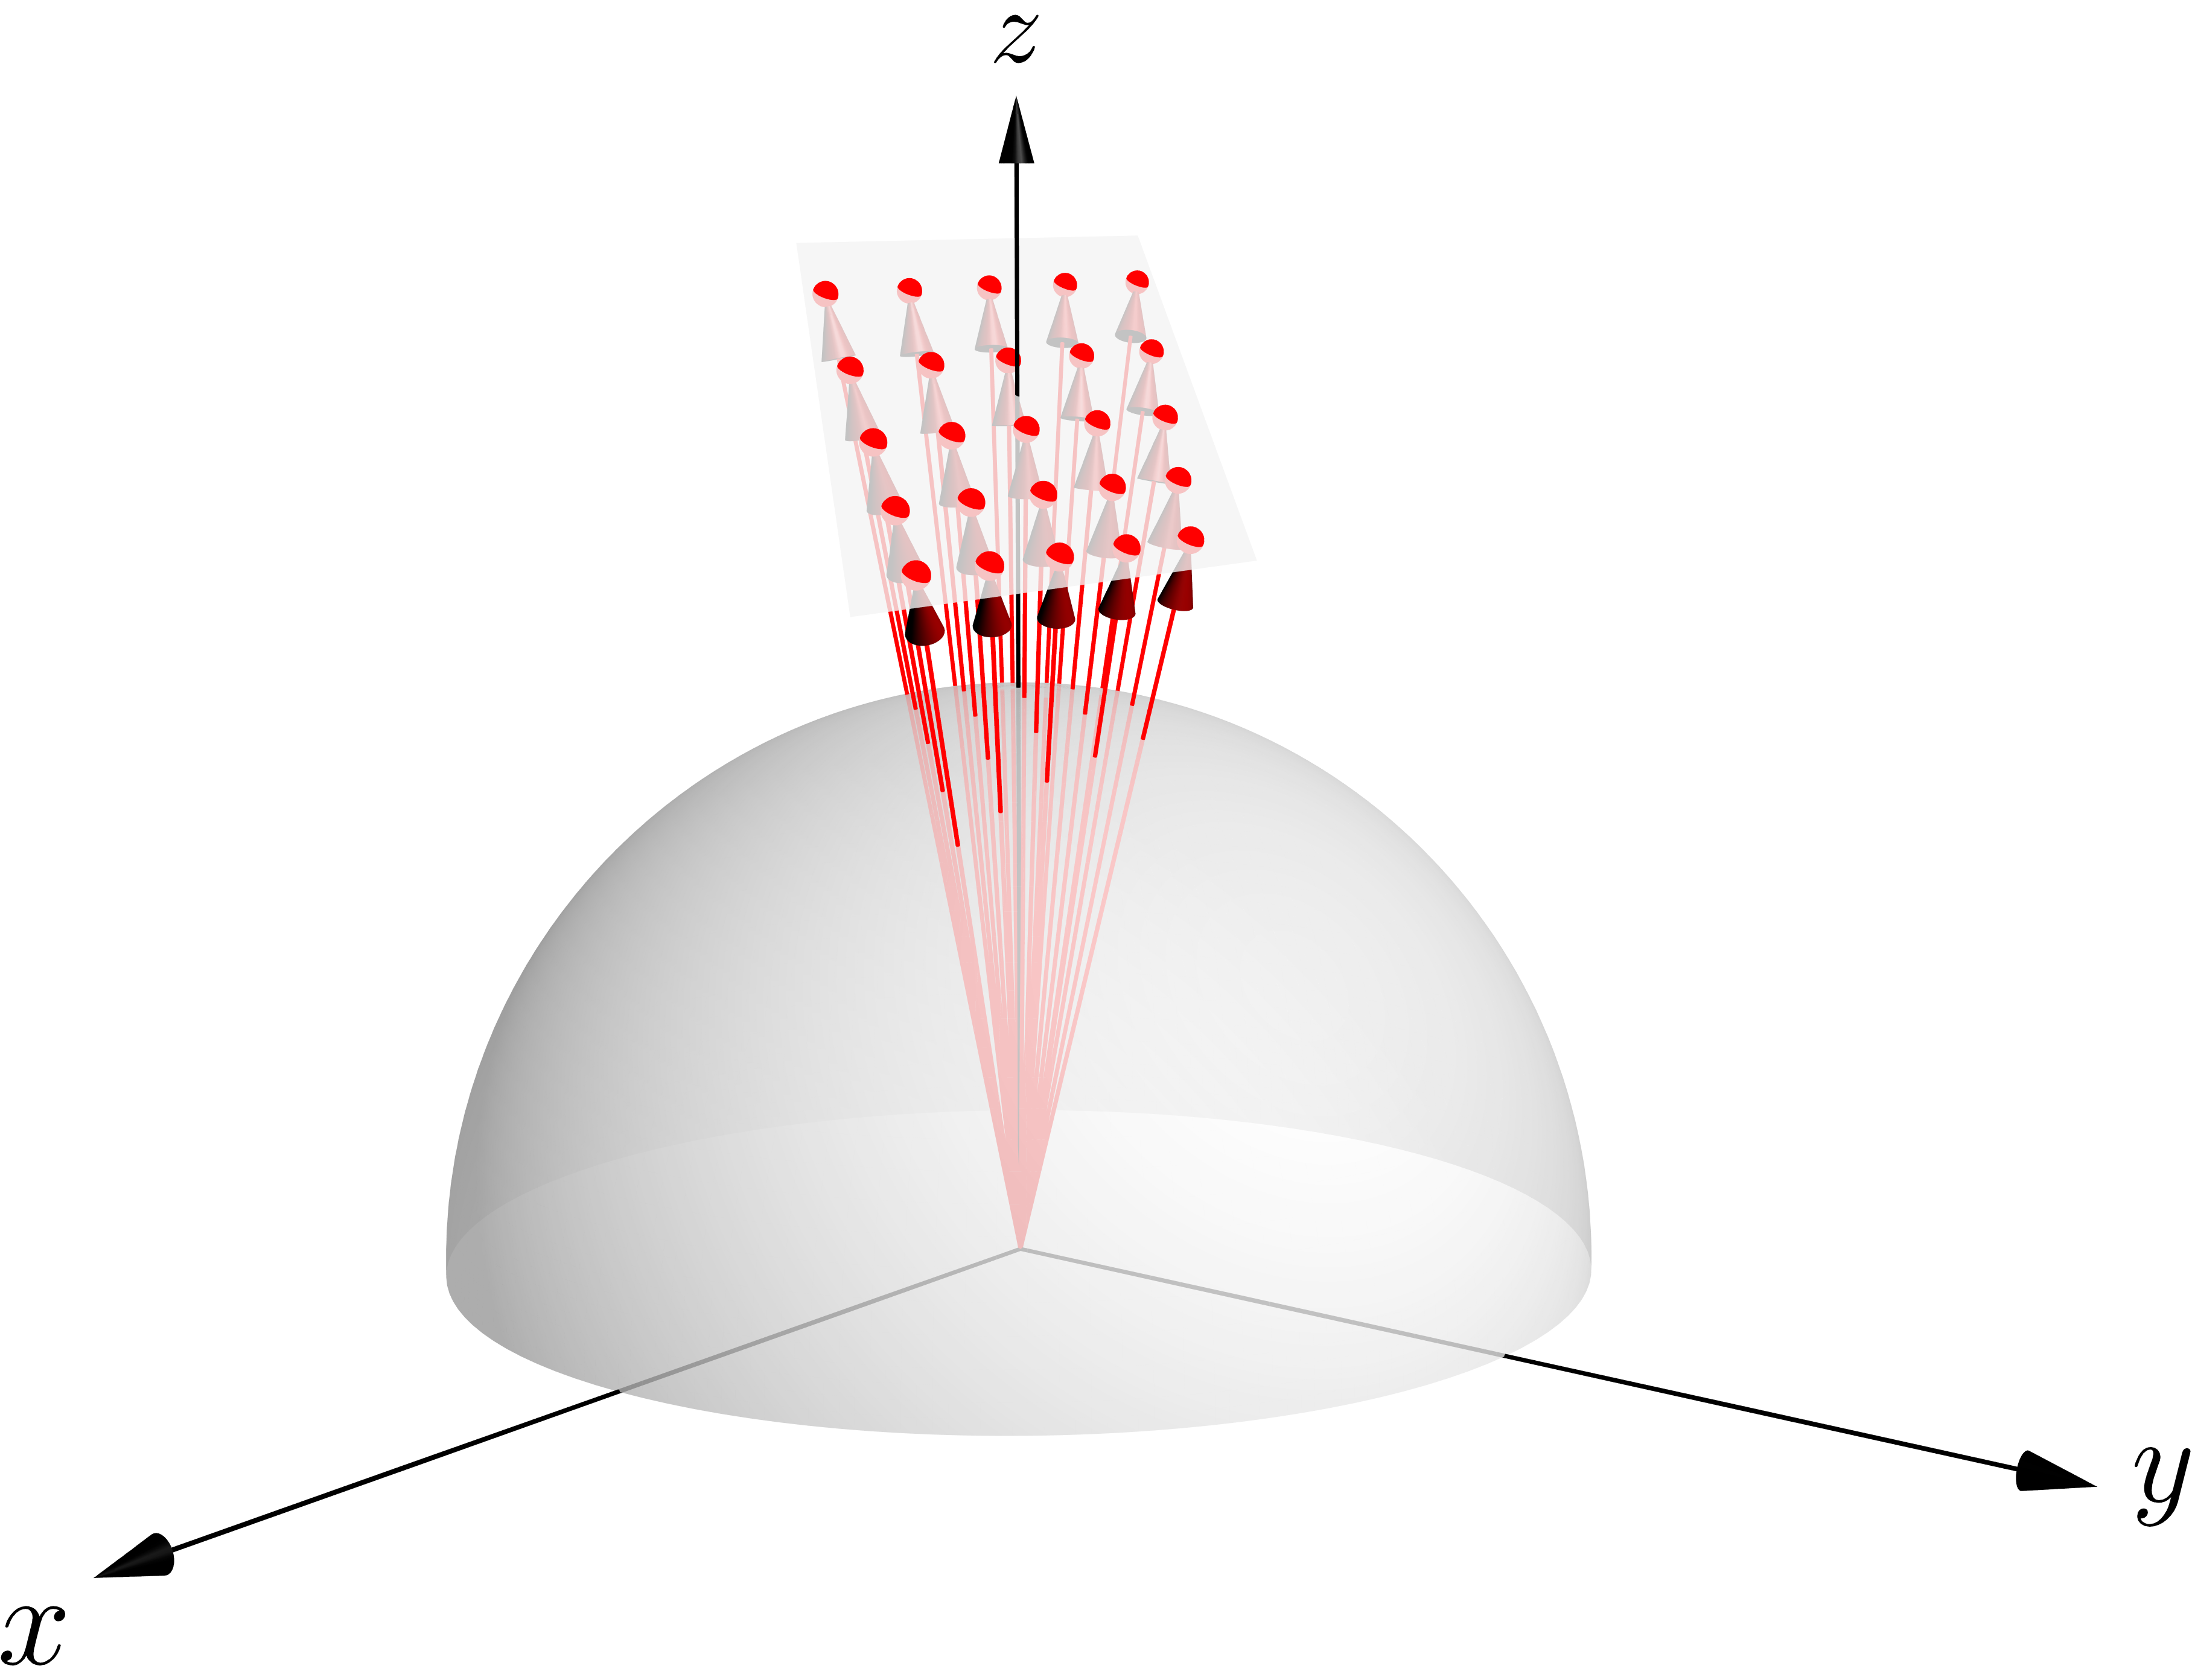
\includegraphics[width=\textwidth]{ltc/sample_transform_before2}
        \label{fig:LTCTransformBefore}
        \caption{Przed przekształceniem}
    \end{subfigure}
    \hspace{0.05\textwidth}
    \begin{subfigure}[t]{0.45\textwidth}
        \centering
        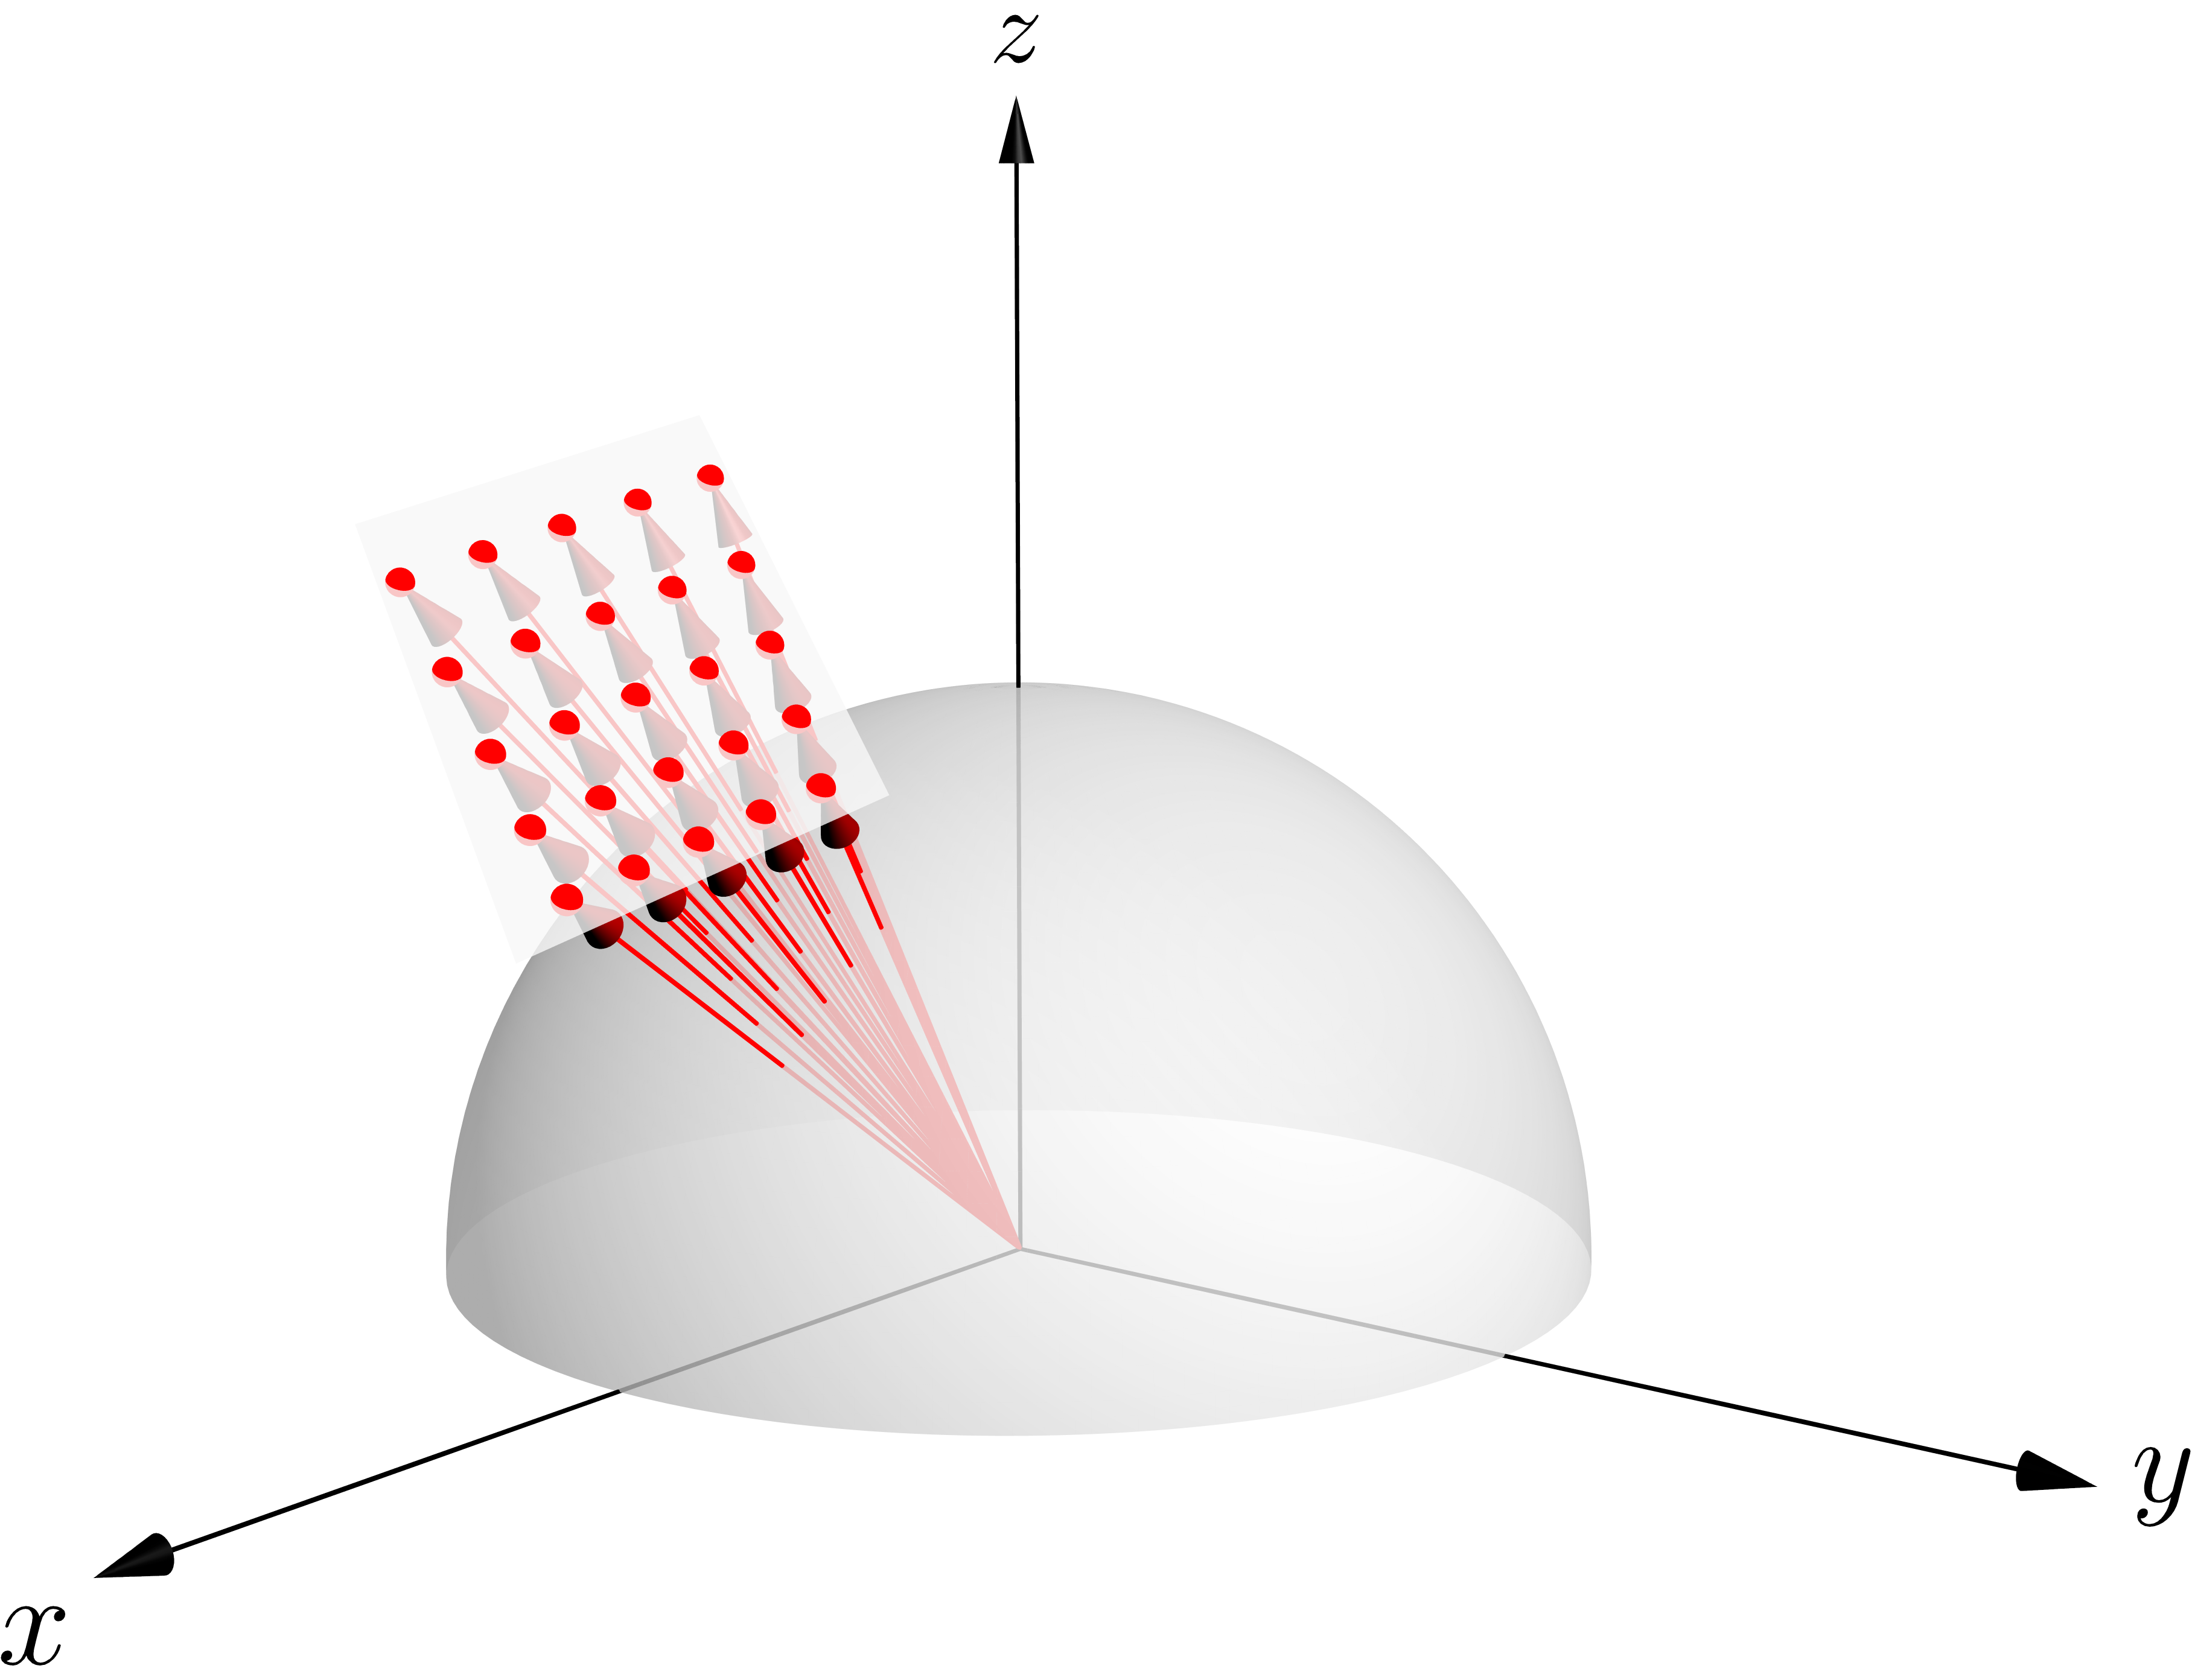
\includegraphics[width=\textwidth]{ltc/sample_transform_after2}
        \label{fig:LTCTransformAfter}
        \caption{Po przekształceniu}
    \end{subfigure}
    
    \caption{Jednoczesne przekształcenie wielokąta i promieni powoduje, że liczba promieni przecinających wielokąt $P$ nie zmienia się. Opracowanie własne.}
    \label{fig:LTCTransformBeforeAfter}
\end{figure}

Rozumowanie można przeprowadzić na odwrót dla przekształcenia $M^{-1}$. Wynika z tego, że jeżeli będziemy w stanie znaleźć prosty rozkład bazowy, który możemy szybko całkować oraz przekształcenie $M^{-1}$ przybliżające rozkład docelowy rozkładem bazowym, to wykorzystując powyższą właściwość możemy przybliżyć wartość całki rozkładu docelowego na wielokącie sferycznym.

%\begin{figure}[ht]
%\missingfigure{Obrazek kilku przekształceń rozkładu LTC}
%\end{figure}

\subsection{Wybór rozkładu bazowego $D_0(\omega)$}

Kolejnym krokiem jest wybór rozkładu bazowego, który po przekształceniu liniowym da nam oczekiwany rozkład spełniający założenia postawione na samym początku.

Rozpocznijmy poszukiwania od najprostszego rozwiązywalnego rozkładu, a mianowicie rozkładu jednorodnego. Jeżeli rozkład $D_A$ przyjmuje taką samą wartość w każdym punkcie to całka na wielokącie sferycznym (ang. \textit{spherical polygon}) jest równoważna kątowi bryłowemu przemnożonym przez odpowiedni stały współczynnik. Istnieje wzór jawny obliczający tą wartość, jest on przedstawiony w publikacjach \cite{Arvo,Snyder}. Bardzo podobnie sytuacja wygląda z półsferą z tym, że wielokąt musi zostać przycięty do horyzontu. Rozkład jednorodny opisany na półsferze możemy opisać równaniem (\ref{eq:LTCUniformD}).
\begin{equation}
D_0(\omega_o=(x_0, y_0, z_0)) = \begin{cases}
  \frac{1}{2\pi} & \text{dla } y_0 \geq 0 \\
  0 & \text{dla } y_0 < 0
\end{cases}
\label{eq:LTCUniformD}
\end{equation}

Niestety, rozkład jednorodny nie jest w stanie modelować żadnych ciekawych zjawisk ze względu na niezmienną naturę.

Nieco bardziej skomplikowanym rozkładem jest przycięty rozkład kosinusowy (ang. \textit{diffuse}, \textit{Lambertian distribution}, \textit{cosine distribution}) opisany równaniem (\ref{eq:LTCCosineD}).
\begin{equation}
D_0(\omega_o=(x_0, y_0, z_0)) = \begin{cases}
  \frac{y_0}{\pi} & \text{dla } y_0 \geq 0 \\
  0 & \text{dla } y_0 < 0
\end{cases}
\label{eq:LTCCosineD}
\end{equation}

Zaletą rozkładu kosinusowego jest fakt, że przechodzi on gładko do $0$ oraz posiada wzór jawny (\ref{eq:ltc_lambert_int}) na wartość całki (\ref{eq:LTCDInt}) wyprowadzony przez Lamberta \cite{Baum}. Obliczanie całki na takim rozkładzie jest z definicji obliczaniem irradiancji wielokąta sferycznego.
\begin{equation}
\begin{gathered}
E(p_1, \ldots, p_n) =
\frac{1}{2\pi}
\sum_{i=0}^{n} {
  \cos^{-1}(\langle p_i, p_j \rangle)
  \left\langle {
    \frac{p_i \times p_j}{\norm{p_i \times p_j}},
    \left[ \begin{matrix} 0 \\ 0 \\ 1 \end{matrix} \right]
  } \right\rangle
} \\
j = (i+1) \text{ mod } n
\end{gathered}
\label{eq:ltc_lambert_int}
\end{equation}

Złożoność wzoru (\ref{eq:ltc_lambert_int}) jest liniowo zależna od stopnia złożoności wielokąta, co umożliwia zastosowanie go w aplikacjach czasu rzeczywistego.

Istnieją również inne potencjalne rozkłady bazowe, ale niestety, w większości przypadków nie nadają się one do zastosowania praktycznego. Rozkłady opisywane przez sferyczne gaussowskie (ang. \textit{spherical gaussian}) nie posiadają wzoru jawnego, rozkład Phong’a posiada wzór jawny, jednak zmienna złożoność zależna liniowo od wykładnika sprawia, że metoda jest niepraktyczna. Bardziej kompleksowe objaśnienia można znaleźć w pracy \cite{ltc_heitz}.

Z powyższych rozważań, wynika, że przycięty rozkład kosinusowy jest dobrym kandydatem na rozkład bazowy ze względu na swoje właściwości i prostą konstrukcję. Będziemy go wykorzystywać w tym celu w dalszej części pracy i oznaczać $D_0(\omega)$.

\section{Uwzględnienie  normy BRDF i współczynnika Fresnela}

Warto również zauważyć, że wszystkie powyższe rozkłady podstawowe mają postać znormalizowaną tzn. zachodzi warunek (\ref{eq:ltc_norm_condition}).
\begin{equation}
\int_\Omega {
    D_0(\omega_0)
    \dd \omega_0
} = 1
\label{eq:ltc_norm_condition}
\end{equation}

Istotną obserwacją jest to, że jeżeli dany materiał pochłania dużą część energii w trakcie odbicia, zastosowanie tej metody w sposób bezpośredni nie wystarczy do uzyskania satysfakcjonujących rezultatów. Ze względu na zjawiska geometryczne, wspomniane w poprzednich rozdziałach, może okazać się, że zachodzi nierówność (\ref{eq:ltc_energy_loss}).
\begin{equation}
    \int_{\Omega} {
        f_r(\omega_i, \omega_o) \cos\theta_i 
        \dd \omega_i
    } < 1
\label{eq:ltc_energy_loss}
\end{equation}

Autor pracy \cite{LTCFresnelApprox} zaleca, aby zachować wartość lewej strony nierówności (\ref{eq:ltc_energy_loss}) razem z dopasowaniem tak, abyśmy mogli przeskalować odpowiedź $D_0(\omega)$, aby zachować proporcję. Oznaczmy lewą stronę nierówności (\ref{eq:ltc_energy_loss}) przez $n_D$.
\begin{equation}
n_D =
\int_{\Omega} {
    f_r(\omega_i, \omega_o) \cos\theta_i 
    \dd \omega_i
}
\label{eq:ltc_nd_def}
\end{equation}

W wielu modelach występuje również współczynnik Fresnela, najczęściej sterowany parametrem materiałowym $F_0$. W takim przypadku, chcielibyśmy uzależnić normę skalującą wartość maksymalną całki rozkładu również od $F_0$. W tym celu skorzystamy z aproksymacji Schlicka do przekształcenia równania renderingu do formy (\ref{eq:ltc_norm_fresnel_start}), która będzie nadawała się do obliczeń.
\begin{equation}
\begin{aligned}
\int_{\Omega} &{
    F(\omega_i, \omega_o)
    f_r(\omega_i, \omega_o) 
    \cos\theta_i 
    \dd \omega_i
} = \\
&= \int_{\Omega} {
    \left[
        F_0 + (1-F_0)(1 - \omega_v \cdot m)^5
    \right]
    f_r(\omega_i, \omega_o) 
    \cos\theta_i 
    \dd \omega_i
} = \\
&= F_0 \int_{\Omega} {
    f_r(\omega_i, \omega_o) 
    \cos\theta_i 
    \dd \omega_i
} + (1-F_0) \int_{\Omega} {
    (1 - \omega_v \cdot m)^5
    f_r(\omega_i, \omega_o) 
    \cos\theta_i 
    \dd \omega_i
}
\end{aligned}
\label{eq:ltc_norm_fresnel_start}
\end{equation}

Oznaczając drugą całkę z ostatniego wyrażenia równania (\ref{eq:ltc_norm_fresnel_start}) symbolem $f_D$ (\ref{eq:ltc_fd_def}) oraz podstawiając $n_D$ otrzymamy finalną wartość normy skalującej (\ref{eq:ltc_final_fresnel_norm}). Stałe $n_D$ oraz $f_D$ powinny zostać wyznaczone podczas szukania optymalnej macierzy $M$ i zapisane razem z nią do późniejszego użycia.

\begin{equation}
f_D = \int_{\Omega} {
    (1 - \omega_v \cdot m)^5
    f_r(\omega_i, \omega_o) 
    \cos\theta_i 
    \dd \omega_i
}
\label{eq:ltc_fd_def}
\end{equation}

\begin{equation}
    F_0 n_D + (1-F_0) f_D 
\label{eq:ltc_final_fresnel_norm}
\end{equation}

\section{Wybór przekształcenia liniowego}

Ostatnim zadaniem jest wybór przekształcenia liniowego, którego będziemy używać do formowania naszego przybliżenia. Dla materiału izotropowego, funkcja BRDF zależy tylko i wyłącznie od kąta obserwacji, a zatem od wektora $V = (\sin\theta, 0, \cos\theta)$ oraz współczynnika chropowatości $\alpha$.

Wróćmy do efektów, które chcemy wymodelować. Pierwszym, najprostszym z nich jest kontrola chropowatości za pomocą współczynnika $\alpha$, która może zostać zrealizowana poprzez skalowanie niejednorodne próbek, ale jednorodne w płaszczyźnie $XY$ (\ref{eq:ltc_uniform_xy_scale}) (rys. \ref{fig:LTCEqualScale}).
\begin{equation}
M_{\alpha} =
\begin{bmatrix}
  \lambda & 0 & 0 \\
  0 & \lambda & 0 \\
  0 & 0 & 1
\end{bmatrix}
\label{eq:ltc_uniform_xy_scale}
\end{equation}

\begin{figure}[h]
\centering
    \begin{subfigure}[t]{0.25\textwidth}
        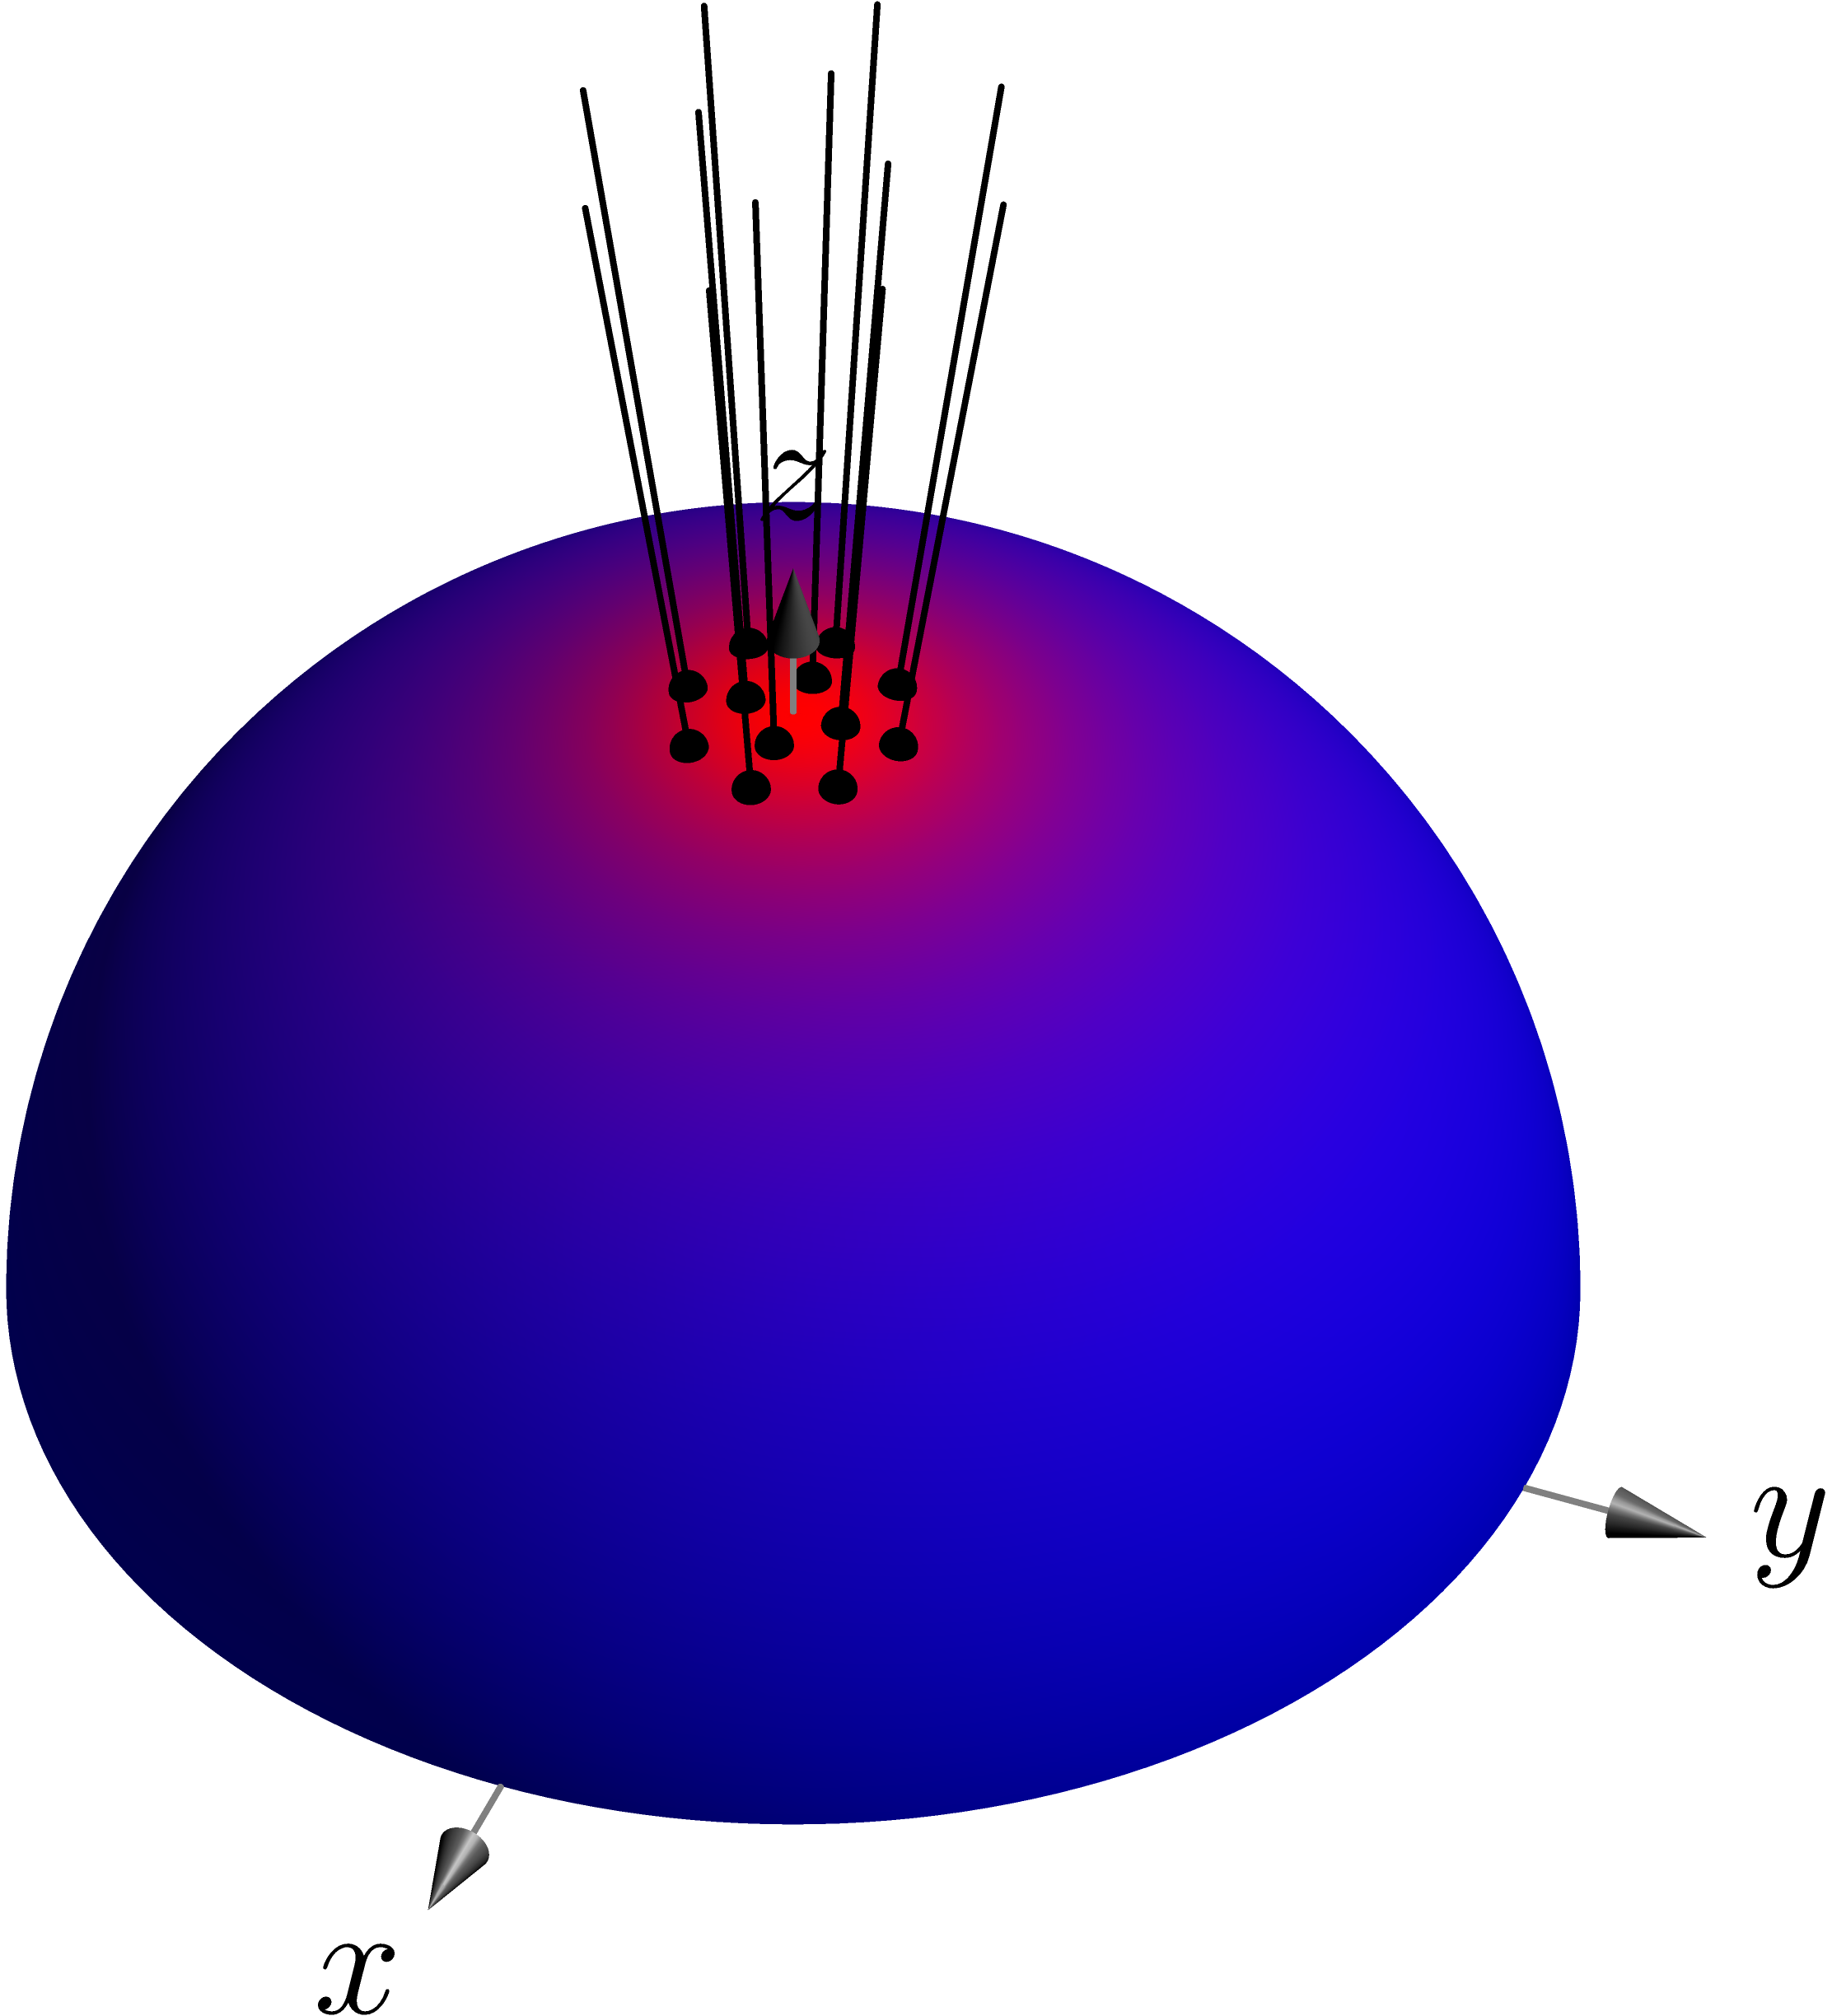
\includegraphics[height=5cm]{ltc/cosine_dist_scale.png}
        \caption{Skalowanie jednorodne.}
        \label{fig:LTCEqualScale}
    \end{subfigure}
    \hspace{0.03\textwidth}
    \begin{subfigure}[t]{0.25\textwidth}
        \centering
        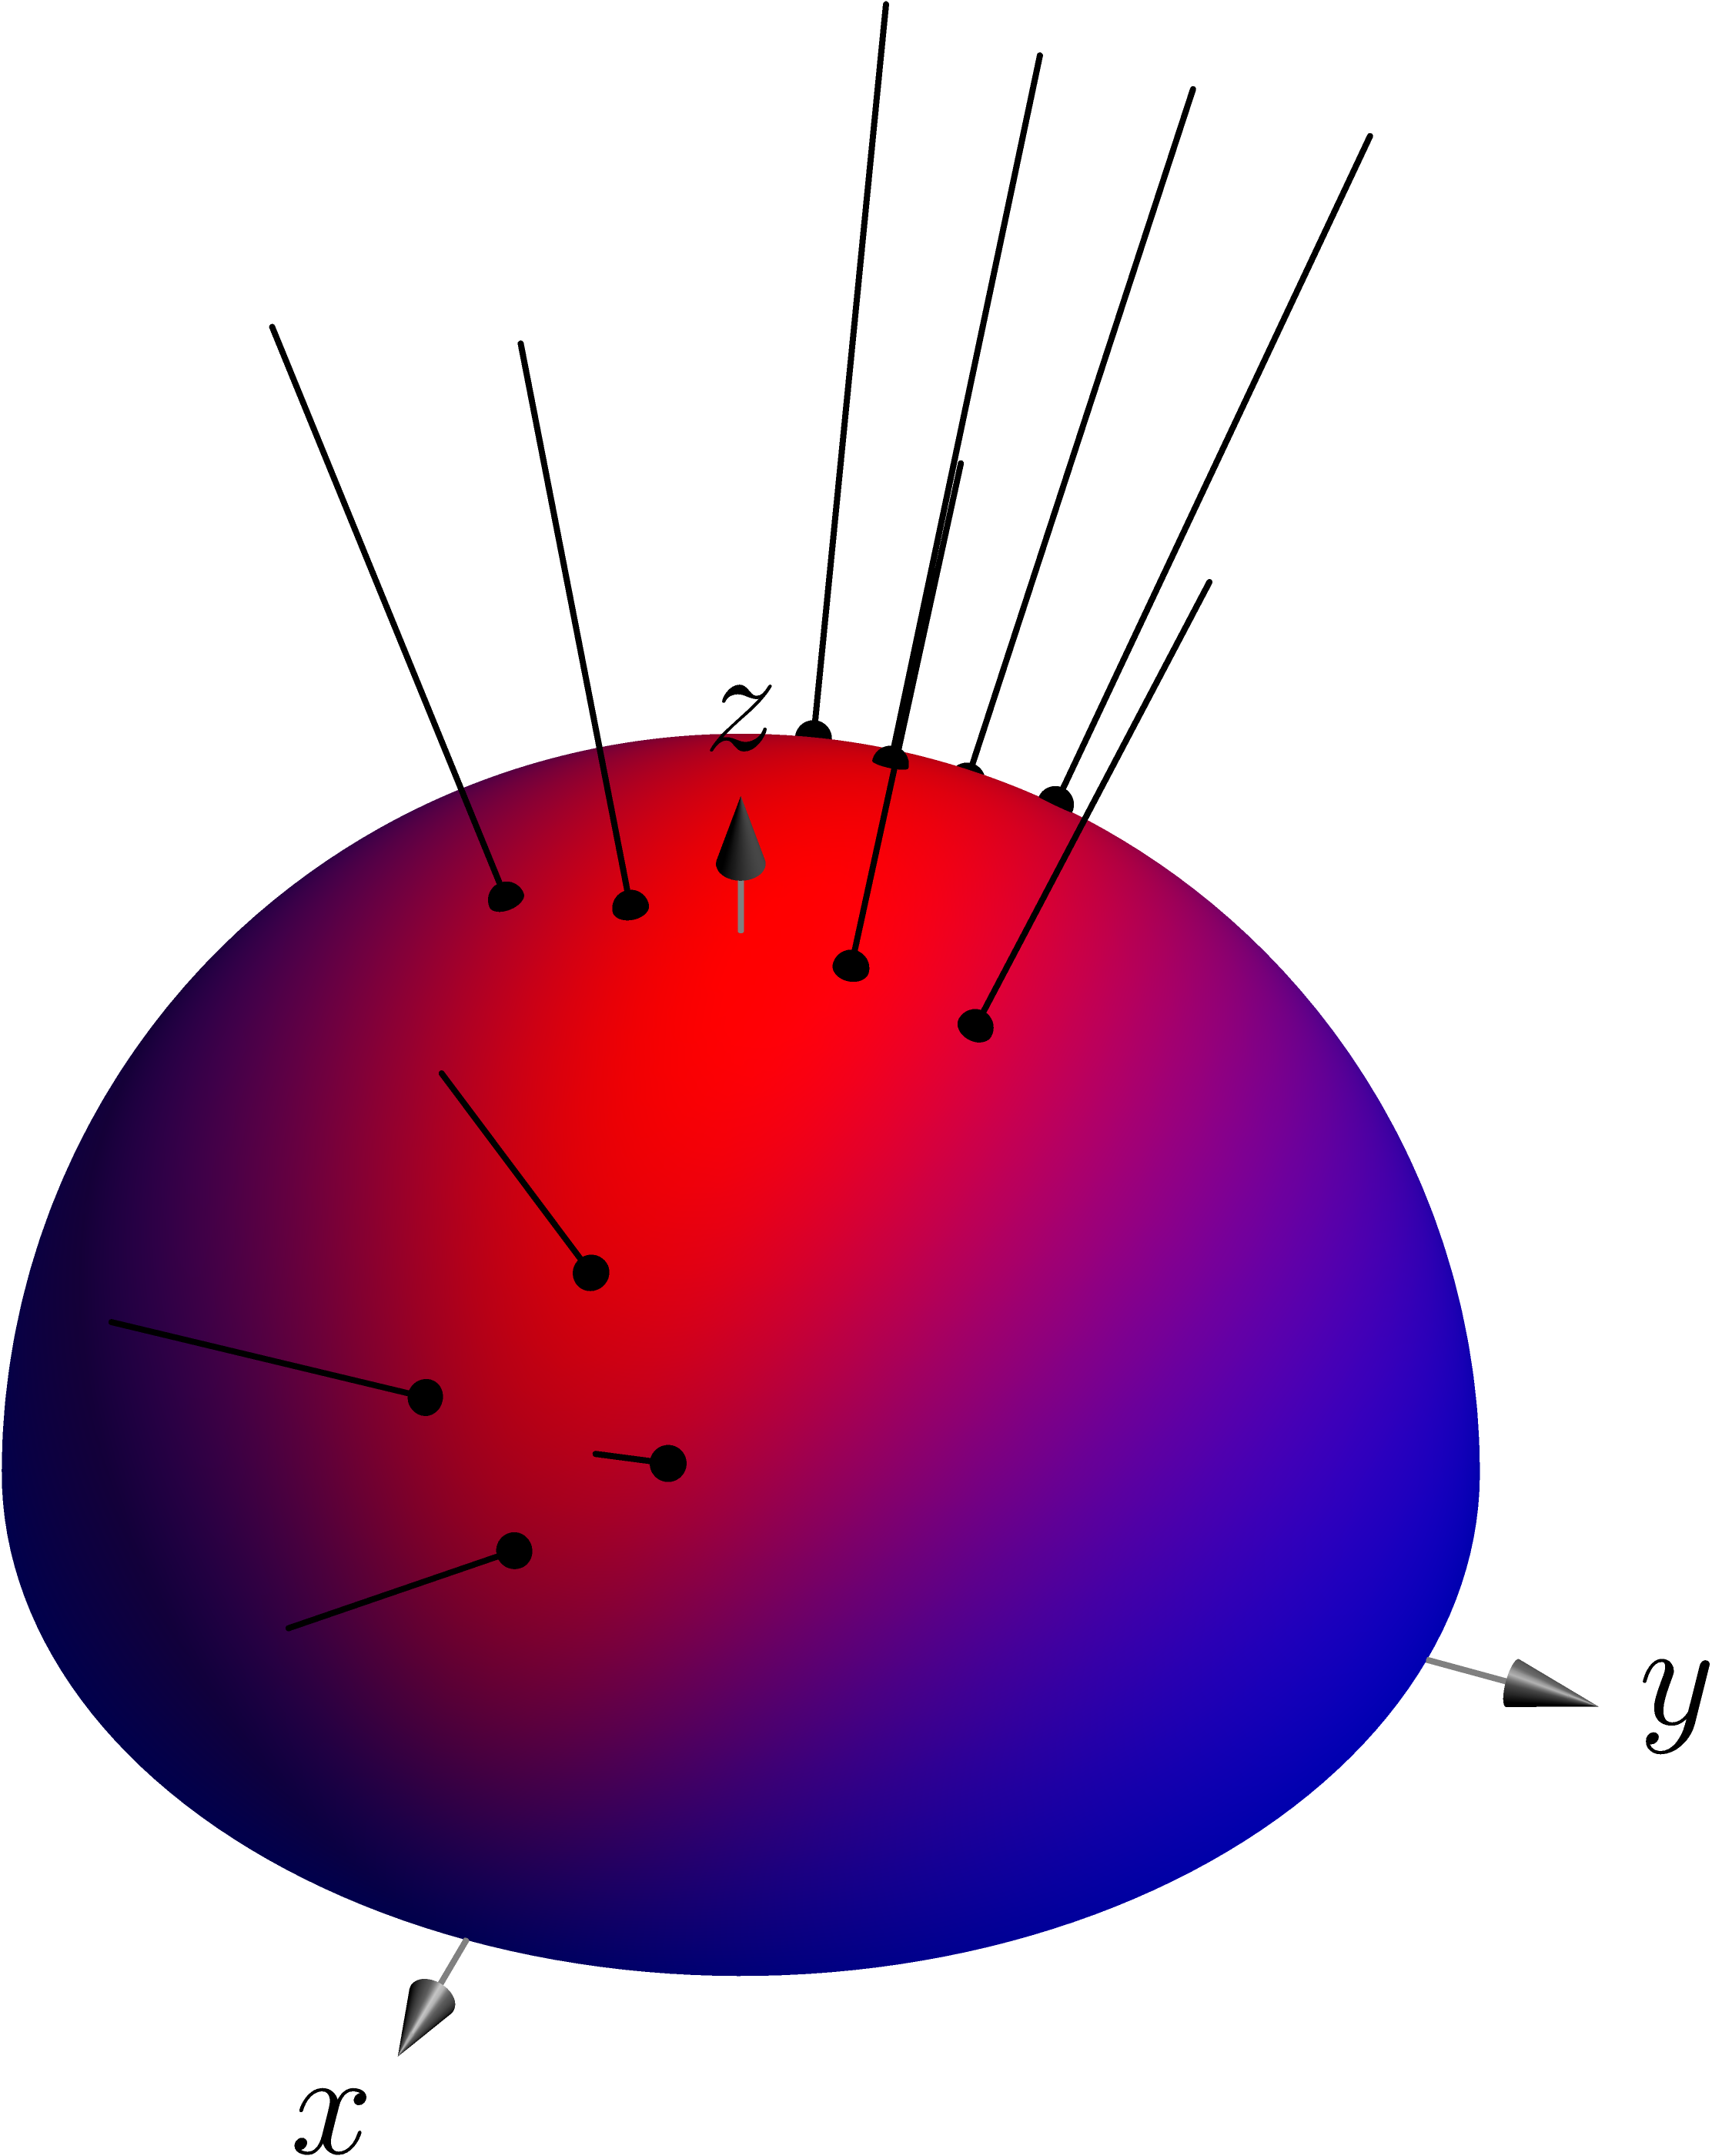
\includegraphics[height=5cm]{ltc/cosine_dist_scale_aniso.png}
        \caption{Skalowanie niejednorodne.}
        \label{fig:LTCAnisoScale}
    \end{subfigure}
    \hspace{0.03\textwidth}
    \begin{subfigure}[t]{0.25\textwidth}
        \centering
        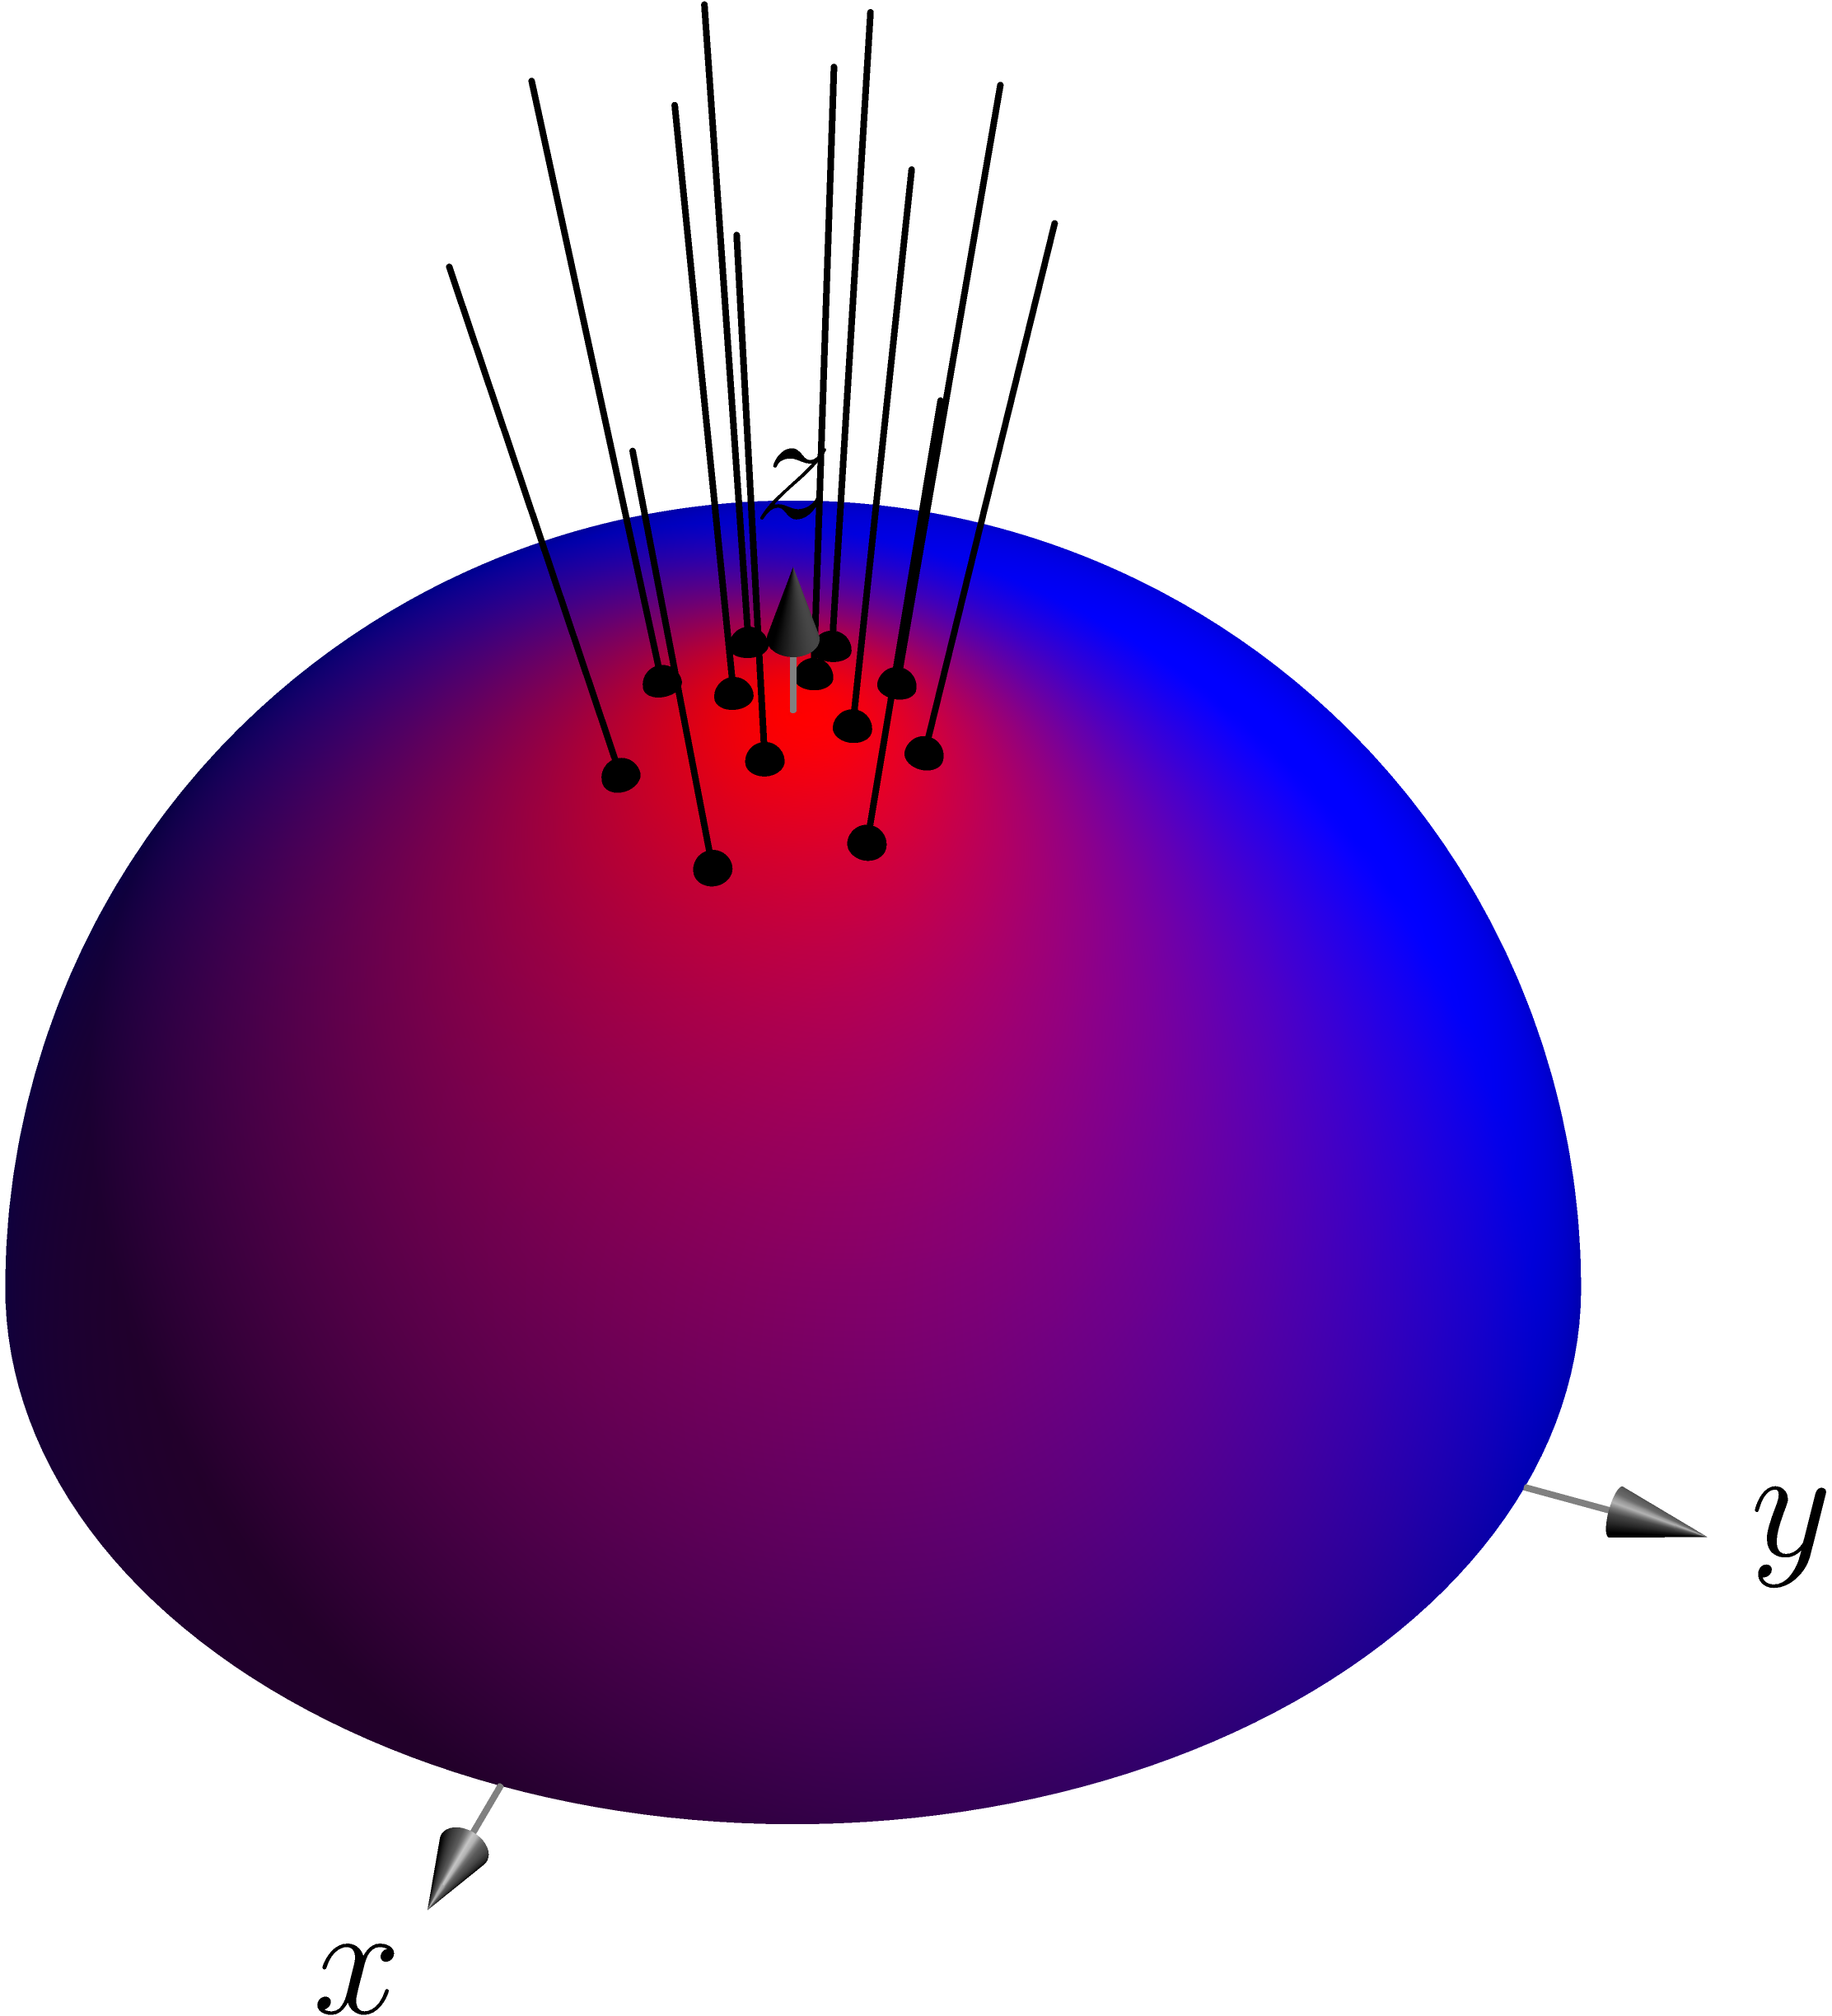
\includegraphics[height=5cm]{ltc/cosine_dist_skew.png}
        \caption{Przekształcenie skośne.}
        \label{fig:LTCSkew}
    \end{subfigure}
    \caption{Przekształcenia bazowe wykorzystane do przybliżania dowolnego rozkładu rozkładem lambertowskim. Opracowanie własne.}
    \label{fig:LTCTransforms}
\end{figure}

Anizotropia powstająca w przy dużych kątach obserwacji może zostać zrealizowana poprzez skalowanie niejednorodne w płaszczyźnie $XY$ (\ref{eq:ltc_nonuniform_xy_scale}) (rys. \ref{fig:LTCAnisoScale}).
\begin{equation}
M_{\text{aniso}} =
\begin{bmatrix}
  \lambda_x & 0 & 0 \\
  0 & \lambda_y & 0 \\
  0 & 0 & 1
\end{bmatrix}
\label{eq:ltc_nonuniform_xy_scale}
\end{equation}

Zjawisko maksimum poza kątem odbicia przy rosnącej chropowatości może zostać zasymulowane poprzez wykorzystanie z macierzy skośnej (\ref{eq:ltc_skew}) (rys. \ref{fig:LTCSkew}).
\begin{equation}
M_{\text{skew}} =
\begin{bmatrix}
  1 & 0 & 0 \\
  0 & 1 & 0 \\
  \lambda_{s} & 0 & 1
\end{bmatrix}
\label{eq:ltc_skew}
\end{equation}

Przekształcenia (\ref{eq:ltc_uniform_xy_scale}), (\ref{eq:ltc_nonuniform_xy_scale}) oraz (\ref{eq:ltc_skew}) dają nam możliwość precyzyjnego modelowania spójnych rozkładów o prostych, ale wystarczających do naszych zastosowań kształtach. Po złożeniu tych macierzy otrzymujemy przekształcenie kształtujące rozkład (\ref{eq:ltc_mtx_prec}).
\begin{equation}
\begin{aligned}
M_{\text{precise}} &=
\begin{bmatrix}
1 & 0 & \lambda_{\text{skew}} \\
0 & 1 & 0 \\
0 & 0 & 1
\end{bmatrix}
\begin{bmatrix}
\lambda_x & 0 & 0 \\
0 & \lambda_y & 0 \\
0 & 0 & 1
\end{bmatrix}
\begin{bmatrix}
\lambda & 0 & 0 \\
0 & \lambda & 0 \\
0 & 0 & 1
\end{bmatrix} 
=
\\
&=
\begin{bmatrix}
\lambda\lambda_x & 0 & \lambda_{\text{skew}} \\
0 & \lambda\lambda_y & 0 \\
0 & 0 & 1
\end{bmatrix}
\stackrel{\text{ozn.}}{=}
\begin{bmatrix}
a & 0 & c \\
0 & b & 0 \\
0 & 0 & 1
\end{bmatrix}
\end{aligned}
\label{eq:ltc_mtx_prec}
\end{equation}

Ostatnią operacją, którą potrzebujemy do precyzyjnego dopasowania rozkładu jest rotacja wokół osi $Y$ (\ref{eq:ltc_rot_y}), pozwalająca nam na dokładne ułożenie uformowanego rozkładu, tak, aby pokryć kierunki o najwyższej wartości (kierunki dominujące).
\begin{equation}
M_{\text{rot}} =
\begin{bmatrix}
\cos\theta_d  & 0     & \sin\theta_d \\
0           & 1     & 0 \\
-\sin\theta_d & 0     & \cos\theta_d
\end{bmatrix}
\label{eq:ltc_rot_y}
\end{equation}

Mnożąc macierz rotacji oraz macierz formującą otrzymamy finalną macierz $M$  (\ref{eq:ltc_mtx_final}).
\begin{equation}
M = M_{\text{rot}} M_{\text{precise}} = \begin{bmatrix}
a\cos\theta_d & 0 & c\cos\theta_d + \sin\theta_d \\
0 & b & 0 \\
-a\sin\theta_d & 0 & \cos\theta_d - c \sin\theta_d
\end{bmatrix} = \begin{bmatrix}
m_{11} & 0 & m_{31} \\
0 & m_{22} & 0 \\
m_{13} & 0 & m_{33}
\end{bmatrix}
\label{eq:ltc_mtx_final}
\end{equation}

Macierz $M$ zawiera cztery niewiadome $a$, $b$, $c$, $\theta_d$, które będziemy wyznaczać metodami numerycznymi. Wykorzystamy technikę dopasowywania danych przeprowadzoną jednokrotnie w formie przetwarzania wstępnego i wykorzystamy gotowe rezultaty podczas rysowania sceny.

Publikacja \cite{ltc_heitz} sugeruje znormalizowanie macierzy tak, aby $m_{33}=1$, ale powoduje to problemy z interpolacją między poszczególnymi przekształceniami w stanach pośrednich. W prezentacji \cite{LTCJourneyPresentation} można znaleźć wyjaśnienie i przykłady problemów niesionych przez te rozwiązanie.

Macierz $M$ ze specyfiki metody musi być odwracalna, zatem: $\det M \neq 0 \Rightarrow ab \neq 0$. Wprowadzimy dodatkowe założenie, że parametry $a$ i $b$ są dodatnie, ze względu na to, że ujemny parametr będzie oznaczał odbicie lustrzane względem osi. W ten sposób również zagwarantujemy poprawność znalezionego rozwiązania.

\section{Dopasowywanie rozkładu}

W celu dopasowania przekształcenia liniowego dla danych $\alpha$ i $\theta$ wykorzystamy algorytm optymalizacji numerycznej.

W celu przyśpieszenia dopasowywania znajdziemy najpierw kierunek dominujący $\omega_d$ (\ref{eq:ltc_wd_def}), normę $n_D$ i współczynnik $f_D$ przybliżanego rozkładu. Dane te umożliwią nam wstępne ustawienie rozkładu bazowego tak, aby najważniejsze kierunki tych rozkładów pokryły oraz przy okazji poznamy normy oryginalnego rozkładu ($n_D$ i $f_D$). Informacje te są możliwe do wyprowadzenia korzystając z metody Monte Carlo z ważeniem próbek, opisanym przez równania (\ref{eq:ltc_montecarlo_equations}).
    
\begin{equation}
    \omega_d = \left( \sin\theta_d, 0, \cos\theta_d \right)
    \label{eq:ltc_wd_def}
\end{equation}
\noindent 

\begin{equation}
\begin{gathered}
\omega_d
\stackrel{n \rightarrow \infty}{=}
\frac{1}{n} \sum_{i=1}^{n} {
    \frac{
        D_{\text{BRDF}}(\omega_i)
    }{
        \text{pdf}_{\text{BRDF}}(\omega_i)
    }
    \omega_i
}
\\
n_D = \int_{\Omega} D_{\text{BRDF}}(\omega)d\omega
\stackrel{n \rightarrow \infty}{=}
\frac{1}{n} \sum_{i=1}^{n} {
  \frac{
    D_{\text{BRDF}}(\omega_i)
  }{
    \text{pdf}_{\text{BRDF}}(\omega_i)
  }
}
\\
f_D = \int_{\Omega} D_{\text{BRDF}}(\omega)d\omega
\stackrel{n \rightarrow \infty}{=}
\frac{1}{n} \sum_{i=1}^{n} {
    \frac{
        D_{\text{BRDF}}(\omega_i) (1 - \omega_i \cdot h)^5
    }{
        \text{pdf}_{\text{BRDF}}(\omega_i)
    }
}
\end{gathered}
\label{eq:ltc_montecarlo_equations}
\end{equation}

W przypadku anizotropowym chcielibyśmy prowadzić rozważania w pewnej płaszczyźnie ze względu na uproszczenie obliczeń. W naszym przypadku założyliśmy, że $y(\omega_d)=0$. Obliczenie kierunku $\omega_d$ metodą Monte-Carlo może spowodować zajście sprzecznego warunku $y(\omega_d) \neq 0$. Z tego powodu dokonujemy przyciągnięcia wektora do płaszczyzny XZ (\ref{eq:ltc_wd_xz_snap}).

\begin{equation}
\widetilde{\omega}_d = \frac{
    \left( \omega_x,0,\omega_z \right)
  }{
    w_x^2+w_z^2
  }
\label{eq:ltc_wd_xz_snap}
\end{equation}

Kolejnym krokiem jest ustawienie czubka rozkładu kosinusowego w kierunku dominującym $\widetilde{\omega}_d$, czyli zbudowanie układu w którym oś $Z$ będzie pokrywać się z kierunkiem $\widetilde{\omega}_d$. Uzyskana macierz $M_{\text{rot}}$ (\ref{eq:ltc_wd_rot_mtx}) będzie częścią składową finalnej macierzy $M$ (\ref{eq:ltc_mtx_final}).

\begin{equation}
M_{\text{rot}} =
\begin{bmatrix}
  \cos\theta_d  & 0     & \sin\theta_d \\
  0           & 1     & 0 \\
  -\sin\theta_d & 0     & \cos\theta_d
\end{bmatrix}
= \begin{bmatrix}
  \bot {\widetilde{\omega}_d} & Y & \widetilde{\omega}_d
\end{bmatrix}
\label{eq:ltc_wd_rot_mtx}
\end{equation}

Kolejnym krokiem jest ukształtowanie rozkładu do formy uwzględniającej parametry wejściowe i występujące zjawiska tj. chropowatość ($\alpha$), anizotropowość przy dużych kątach obserwacji i efekt skośny (występujący na jednej z osi), co wymaga numerycznego wyznaczenia parametrów $a$, $b$ i $c$ opisanych w poprzednim podrozdziale.

\subsection{Metoda pływającego sympleksu}

Zdefiniujmy nasz problem w postaci problemu optymalizacyjnego. Chcielibyśmy zminimalizować funkcję $f(a,b,c)$, będącą miarą różnicy (błędu) absolutnej pomiędzy oryginalnym rozkładem, a przybliżonym. Mając pewne parametry $a$, $b$, $c$ będące wynikiem kroku algorytmu optymalizacji chcielibyśmy ocenić jakość przybliżenia wyznaczonego przez te parametry. W tym celu stworzymy funkcję błędu (\ref{eq:ltc_error_fn}), która może zostać obliczona z wykorzystaniem techniki MIS opisanej w rozdziale \ref{Chapter:MIS}.

\begin{equation}
f(a,b,c) =
\int_{\Omega} {
    \abs{
        {D_{\text{LTC}}(a, b, c, \omega) - D_{\text{BRDF}}(\omega)}
    }
} \dd \omega
\label{eq:ltc_error_fn}
\end{equation}

Funkcja (\ref{eq:ltc_error_fn}) posiada dwa ograniczenia narzucone przez warunek $\det M \neq 0$, a mianowicie:
  $a > 0 \wedge b > 0$

Oryginalna metoda pływającego sympleksu \cite{NelderMead65} nie posiada mechanizmu dla ograniczeń, ale istnieją techniki pozwalające rozwiązać ten problem. W mojej implementacji wykorzystałem logarytmiczną wewnętrzną (barierową) funkcję kary $p_{\mathbb{L}}(x, \rho)$ (\ref{eq:ltc_penalty_fn_barrier}). Alternatywną funkcją kary jest funkcja hiperboliczna $p_{\mathbb{H}}(x, \rho)$ (\ref{eq:ltc_penalty_fn_hiper}).

\begin{equation}
  p_{\mathbb{L}}(x, \rho) = - \frac{1}{\rho} \sum_{i=1}^{m} \log(-g_i(x))
\label{eq:ltc_penalty_fn_barrier}
\end{equation}
\begin{equation}
  p_{\mathbb{H}}(x, \rho) =
    - \frac{1}{\rho} \sum_{i=1}^{m} \frac{1}{g_i(x)}
\label{eq:ltc_penalty_fn_hiper}
\end{equation}


\section{Cieniowanie sceny}

Kolor danego punktu $p$ obserwowanego pod kątem $\theta$ do normalnej, o chropowatości $\alpha$, oświetlonego światłem powierzchniowym $P$ o stałej luminancji energetycznej $L$ możemy z łatwością wyznaczyć znając już macierz $M$ oraz parametry $n_D$ i $f_D$.

Pierwszym krokiem jest przekształcenie wielokąta $P$ transformacją $M$ do przestrzeni rozkładu bazowego oraz obcięcie go do horyzontu (rys. \ref{fig:QuadClip}). Obcinanie może być zrealizowane przez proste przejście po krawędziach i odrzucenie części dla której zachodzi $z=0$ i łącząc punkty niespójności liniami prostymi (dla tych linii składowa $z$ będzie zawsze równa $0$). Implementacja zastosowana przez \cite{ltc_heitz}, z której również korzysta ta praca, obsługuje każdy przypadek osobno ze względów wydajnościowych i ograniczeń programów cieniujących.

\begin{figure}[h]
    \centering
    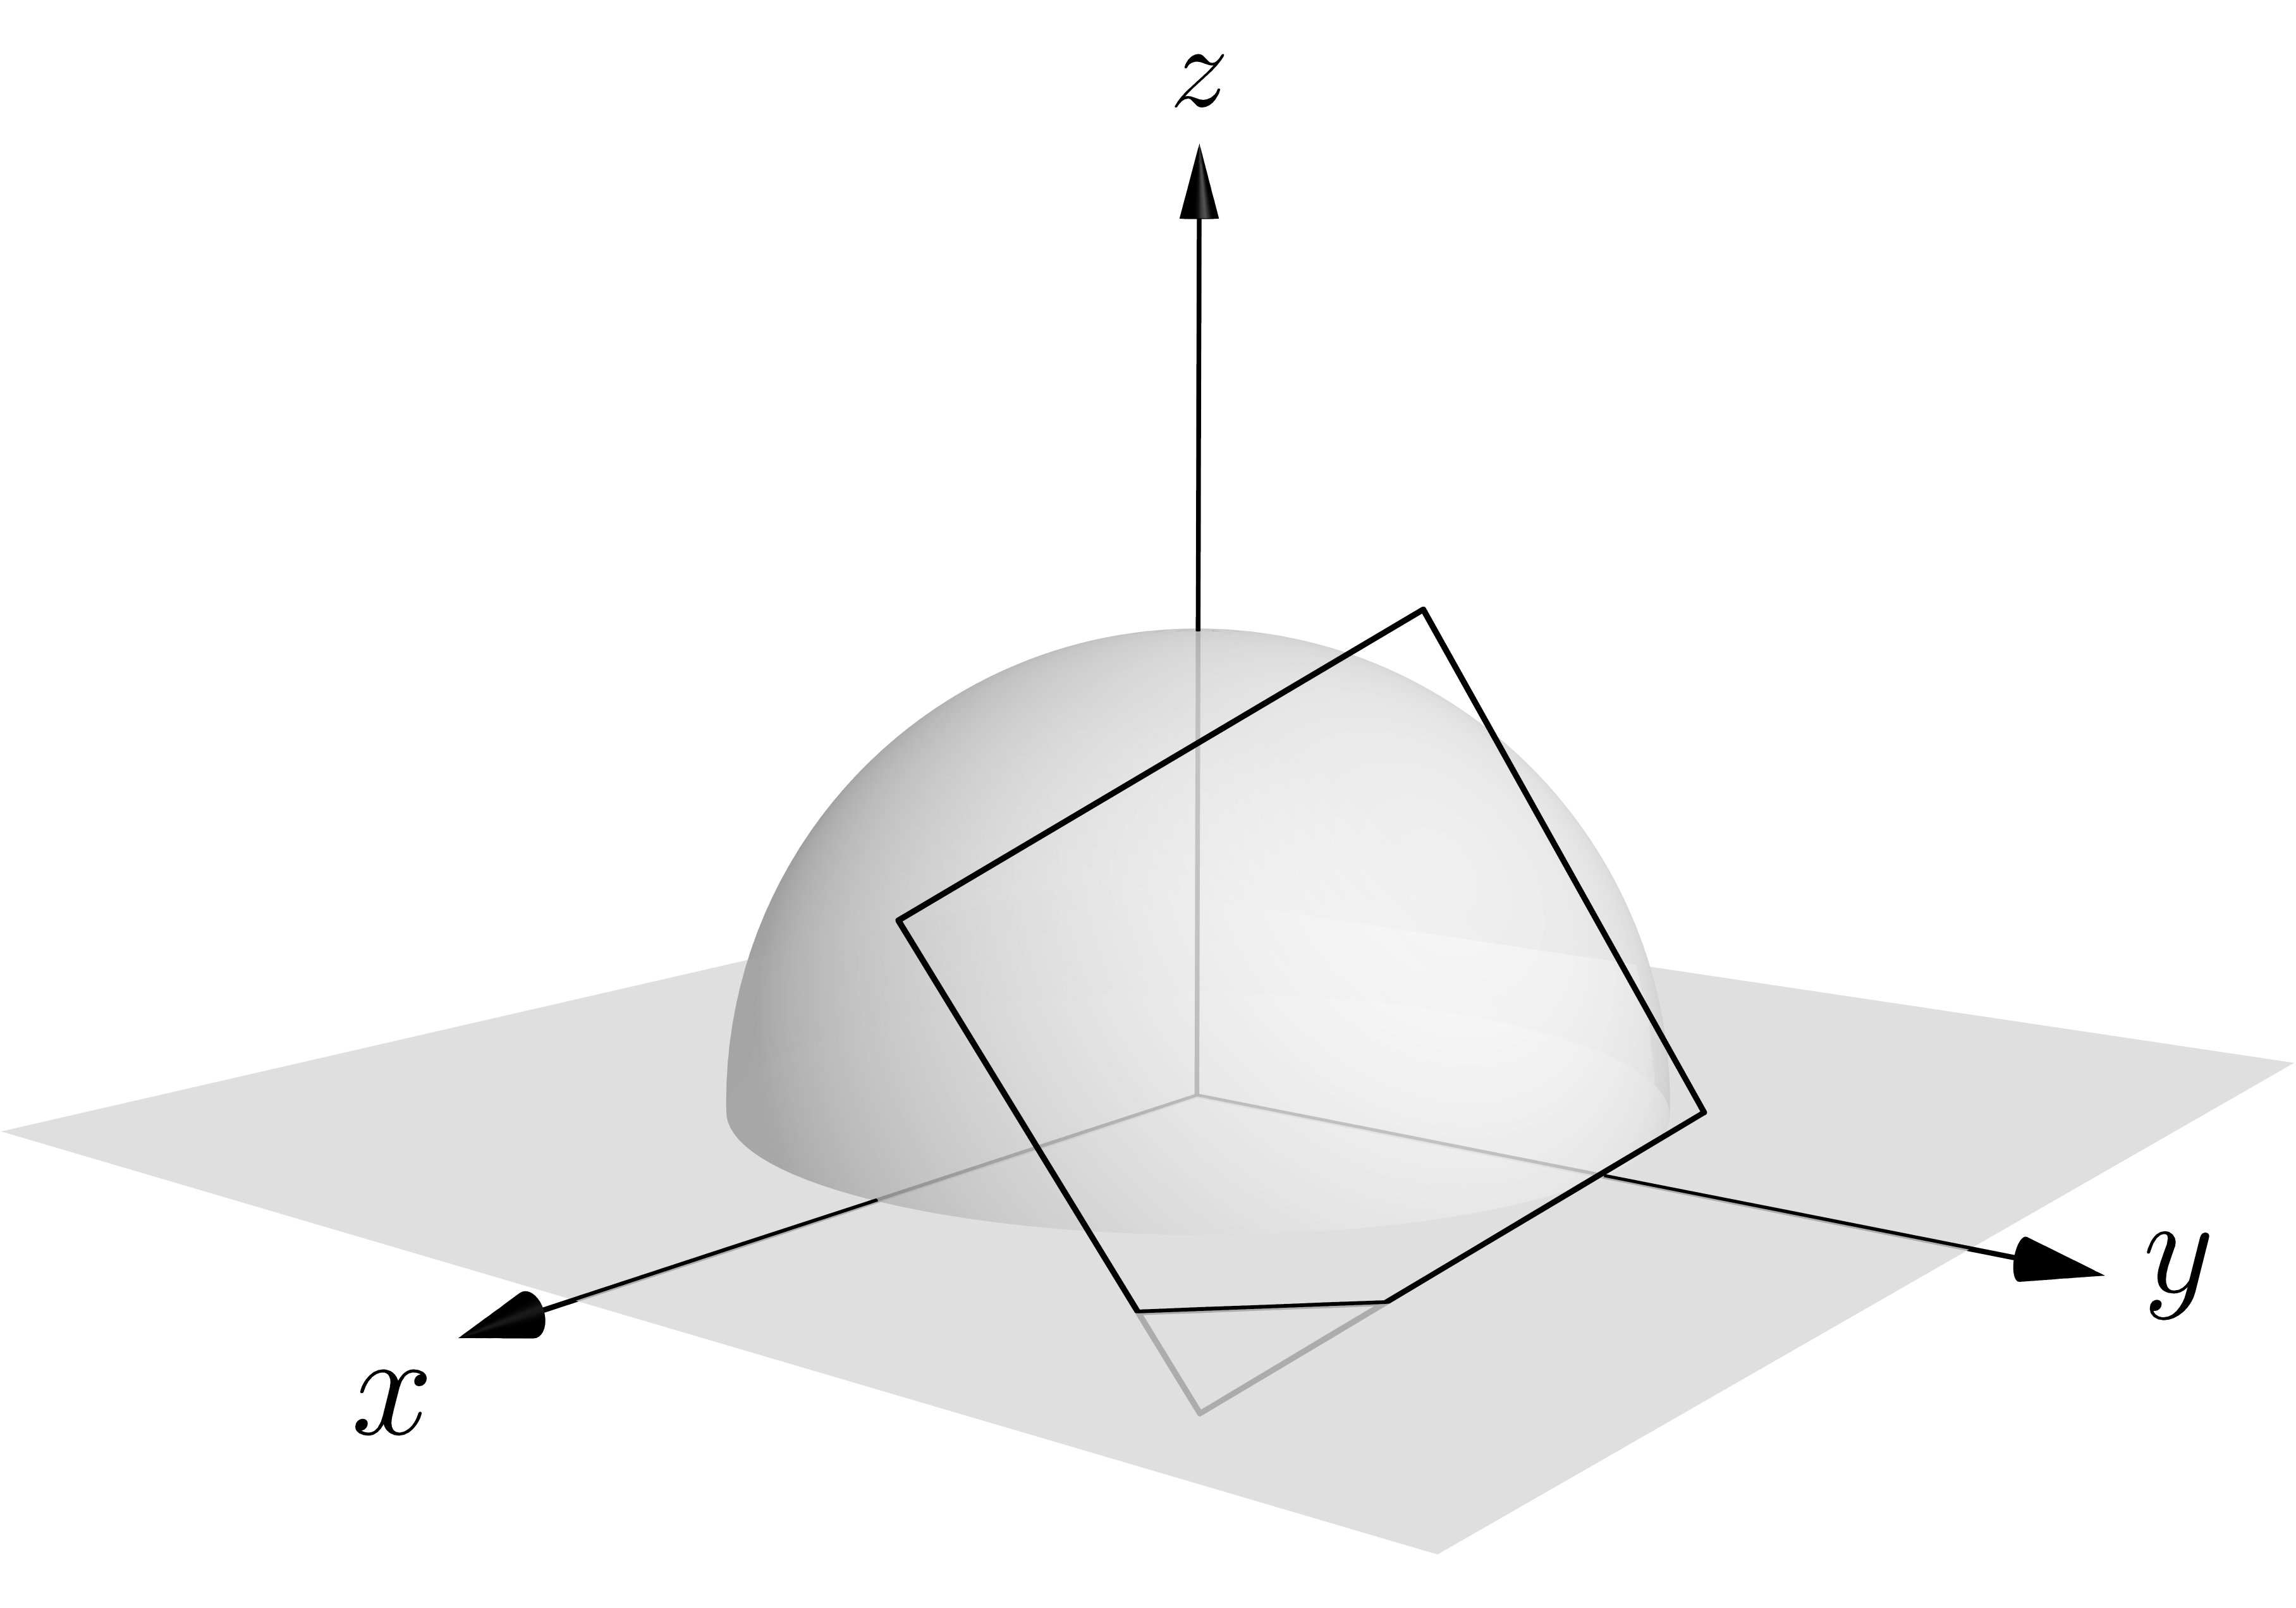
\includegraphics[width=0.6\textwidth]{ltc/quad_clip}
    \caption{Prostokątne źródło światła przycięte do horyzontu. Opracowanie własne.}
    \label{fig:QuadClip}
\end{figure}

Kolejnym krokiem jest obliczenie irradiancji tego wielokąta przy użyciu wzoru   Lamberta (\ref{eq:ltc_lambert_int}). Bezpośrednia implementacja niestety nie da nam oczekiwanych rezultatów, ze względu na przybliżenia zastosowane do implementacji funkcji $\cos^{-1}$ na kartach graficznych. Błąd, mimo że jest niewielki i wystarczający do większości zastosowań, jest zbyt duży do poprawnego wyznaczenia irradiancji wielokąta. W związku z powyższym autorzy \cite{LTCJourneyPresentation} proponują własne przybliżenie.

Okazuje się, że dobre rezultaty daje przybliżenie większej części równania, a mianowicie czynnika\footnote{Użyteczność tej formy wynika z faktu, że $\norm{p_i \times p_j} = \norm{p_i}\:\norm{p_j}\sin\theta$.}: $\frac{\theta}{\sin\theta}$. Metodą prób i błędów autorom udało się dobrać funkcję przybliżającą korzystając z optymalizacji funkcji. Znaleziona funkcja wyznacza dobre przybliżenie dla parametru $\langle p_i, p_j \rangle$ w przedziale $(0,1]$. Wprowadzając oznaczenie $\gamma$ (\ref{eq:ltc_gamma_def}) możemy zapisać równanie (\ref{ltc_gamma_approx_positive}). W przypadku, gdy $\langle p_i, p_j \rangle \in [-1, 0)$, możemy wyznaczyć wartość przybliżenia korzystając z własności (\ref{ltc_gamma_approx_negative}).

\begin{equation}
\gamma = \abs{\cos\theta} = \abs{\langle p_i, p_j \rangle}
\label{eq:ltc_gamma_def}
\end{equation}

\begin{equation}
\frac{\theta}{\sin\theta} = f(\gamma) = \frac{
    5.42031 + \left( 3.12829 + 0.0902326 \gamma \right) \gamma
}{
    3.45068 + \left( 4.18814 + \gamma \right) \gamma
}
\label{ltc_gamma_approx_positive}
\end{equation}

\begin{equation}
    \frac{\pi - \theta}{\sin\left( \pi-\theta \right)} =
    \frac{\pi - \theta}{\sin\theta} = 
    \frac{\pi}{\sqrt{1-\cos^{2}\theta}} - \frac{\theta}{\sin\theta} =
    \frac{\pi}{\sqrt{1-\gamma^2}} - f(\gamma)
\label{ltc_gamma_approx_negative}
\end{equation}

W zależności od tego, czy światło jest dwustronne czy nie, należy wziąć wartość absolutną irradiancji $E$ lub obciąć ją do zera. Do obliczenia końcowej wartości wykorzystujemy czynnik skalujący (\ref{eq:ltc_final_fresnel_norm}). Do obliczenia wpływu czynnika rozproszonego możemy wykorzystać macierz $M = I$ oraz ponownie obliczyć irradiancję wielokąta.

\section{Przechowywanie dopasowywanych danych}

Ze względu na ograniczenia techniczne do zbudowania podglądu przekształceń wykorzystamy równomierną siatkę próbek $n \times n$ na prostokącie $(\alpha, \theta) \in \left[0,1\right] \times \left[0, \frac{\pi}{2}\right]$.

Plik zawierający wyniki dla poszczególnych $\alpha$, $\theta$ przechowuje je w formie dwóch tablic dwuwymiarowych przetworzonych w taki sposób, aby były gotowe do wczytania przez kartkę graficzną bez dodatkowych obliczeń. Dokładny opis formatu pliku znajduje się w rozdziale poświęconym architekturze aplikacji (rozdział \ref{chapter:TODO}).

Pierwsza tekstura zawiera współczynniki $M_{1}^{1}, M_{1}^{3}, M_{2}^{2}, M_{3}^{1}$ w postaci liczb zmiennoprzecinkowych o pojedynczej precyzji. Druga tekstura zawiera pozostały istotny współczynnik, czyli $M_{3}^{3}$, normę referencyjnego BRDF $n_D$ oraz oszacowany współczynnik Fresnela $f_D$.

\end{document}
